% \section{Motivation}

\begin{abstract}
% Off-Policy Evaluation (OPE) in contextual bandits enables assessing new policies using existing data without experimentation. Current OPE methods, such as Inverse Probability Weighting (IPW) and Doubly Robust (DR) estimators, suffer from high variance, particularly when there is low overlap between target and behavior policies or large action and context spaces. In this paper, we propose a novel OPE estimator, the Marginal Ratio (MR) estimator, which focuses on the shift in the marginal distribution of outcomes $Y$ rather than the policies themselves. We theoretically show that the MR estimator is more efficient and has lower variance compared to conventional methods like IPW and DR. Furthermore, we establish a connection between the MR estimator and the state-of-the-art Marginalized Inverse Propensity Score (MIPS) estimator, demonstrating that MR achieves the lowest variance among a generalized family of MIPS estimators. We also demonstrate the applicability of the MR estimator in causal inference settings for estimating Average Treatment Effects (ATE), where it outperforms state-of-the-art methods. Our contributions are supported by theoretical analyses and experiments on synthetic and real-world datasets, highlighting the improved performance of the MR estimator.

% Off-Policy Evaluation (OPE) in contextual bandits is crucial for assessing new policies using existing data without costly experimentation. However, current OPE methods, such as Inverse Probability Weighting (IPW) and Doubly Robust (DR) estimators, suffer from high variance, particularly in cases of low overlap between target and behavior policies or large action and context spaces. In this paper, we introduce a new OPE estimator for contextual bandits, the Marginal Ratio (MR) estimator, which focuses on the shift in the marginal distribution of outcomes $Y$ instead of the policies themselves. Through rigorous theoretical analysis, we demonstrate the benefits of MR estimator compared to conventional methods like IPW and DR in terms of variance reduction. Additionally, we establish a connection between our MR estimator and the state-of-the-art Marginalized Inverse Propensity Score (MIPS) estimator, proving that MR attains the lowest variance among a generalized family of MIPS estimators. We further showcase the versatility of the MR estimator in causal inference settings, where it surpasses current state-of-the-art methods in estimating Average Treatment Effects (ATE). Our extensive experiments on synthetic and real-world datasets corroborate our theoretical findings, emphasizing the superiority of the MR estimator in performance and practical applicability, making it a compelling choice for OPE in contextual bandits.


Off-Policy Evaluation (OPE) in contextual bandits is crucial for assessing new policies using existing data without costly experimentation. However, current OPE methods, such as Inverse Probability Weighting (IPW) and Doubly Robust (DR) estimators, suffer from high variance, particularly in cases of low overlap between target and behavior policies or large action and context spaces. In this paper, we introduce a new OPE estimator for contextual bandits, the Marginal Ratio (MR) estimator, which focuses on the shift in the marginal distribution of outcomes $Y$ instead of the policies themselves. Through rigorous theoretical analysis, we demonstrate the benefits of the MR estimator compared to conventional methods like IPW and DR in terms of variance reduction. Additionally, we establish a connection between the MR estimator and the state-of-the-art Marginalized Inverse Propensity Score (MIPS) estimator, proving that MR achieves lower variance among a generalized family of MIPS estimators. We further illustrate the utility of the MR estimator in causal inference settings, where it exhibits enhanced performance in estimating Average Treatment Effects (ATE). Our experiments on synthetic and real-world datasets corroborate our theoretical findings and highlight the practical advantages of the MR estimator in OPE for contextual bandits. 
\end{abstract}
% \emph{Off-Policy Evaluation (OPE)} evaluates the performance of a new target policy which has not been deployed, only using the available observational data. 
% Various OPE methods have been proposed in the literature \citep{thomas2016data,saito2021evaluating,saito2022off,wang2017optimal}. However, these methods often suffer from high variance, leading to unreliable estimates when the data size is not large. Many methods have thus been proposed to alleviate this problem using methods such as Double robust methods \citep{dudik2014doubly}, however, the variance in these estimators can still increase as the variance of contexts or actions increases. In this paper, we propose \emph{marginal ratio (MR)} estimator, an alternative method of off-policy evaluation which does not depend on the context/action variance, and only considers the shift in distribution of outcomes as a result of the policy shift. We prove that our proposed OPE estimator has lower variance compared to the most commonly used OPE estimator, the Inverse Probability Weighting (IPW) estimator.
\section{Introduction} 
% \begin{itemize}
%     \item In contextual bandits the goal is to take an action A based on some contextual information X to then maximize the outcome Y.
%     \item This setup is common in many real-world settings such as healthcare, personalized recommendation systems, and online advertising, etc \citep{li2010contextual, bastani2019online, xu2020contextual}, where the goal is to take actions i.e. taking a drug or recommending an item which subsequently leads to a desirable outcome such as the patients health or click in recommendations.
%     \item However a question arises when we want to change and update the policy. Hence, in the recent years much of research has been spent on evaluating how a new policy will do based on the collected data up to now. In particular, this is also known as the field of off-policy evaluation.
% \end{itemize}
% \begin{wrapfigure}{r}{0.5\textwidth}
%     \centering
%     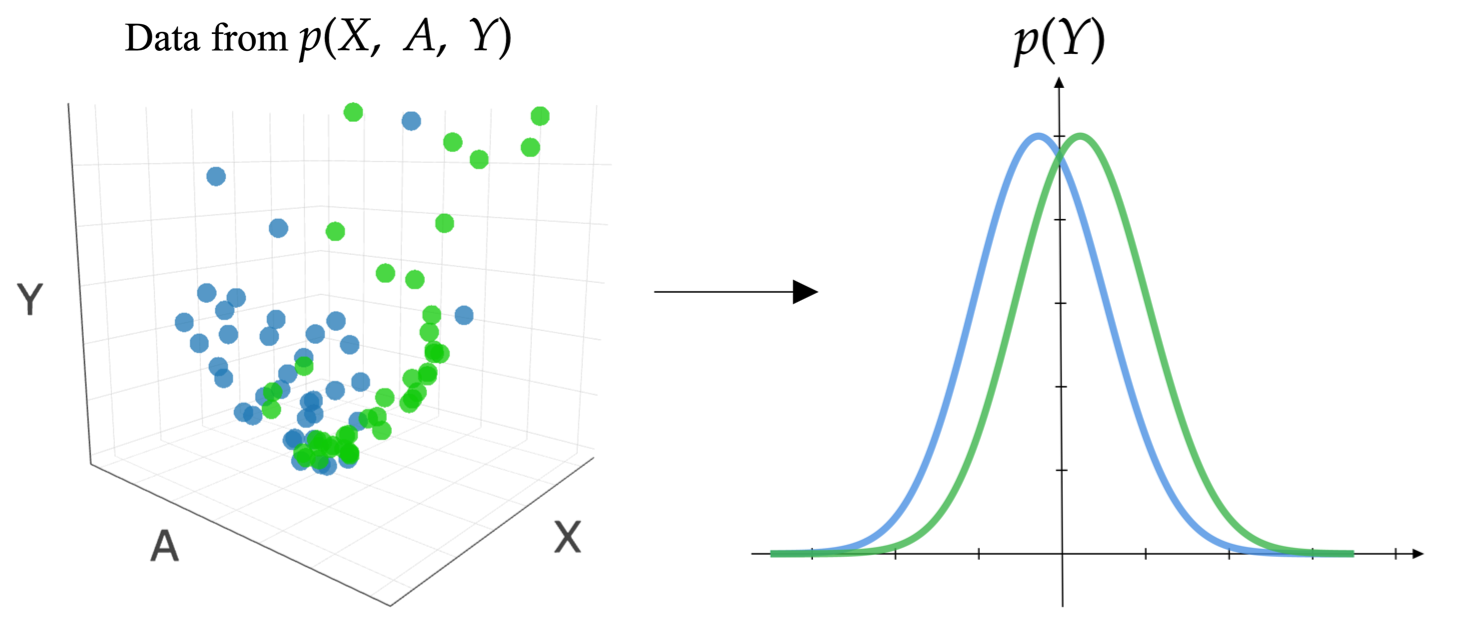
\includegraphics[width=0.5\textwidth]{figures/mr/main_pic.png}
%     \caption{Caption}
%     % \vspace{-1cm}
%     \label{fig:my_label}
% \end{wrapfigure}
In contextual bandits, the objective is to select an action $A$, guided by contextual information $X$, to maximize the resulting outcome $Y$. This paradigm is prevalent in many real-world applications such as healthcare, personalized recommendation systems, or online advertising \citep{li2010contextual, bastani2019online, xu2020contextual}. The objective is to perform actions, such as prescribing medication or recommending items, which lead to desired outcomes like improved patient health or higher click-through rates. Nonetheless, updating the policy presents challenges, as na\"ively implementing a new, untested policy may raise ethical or financial concerns. For instance, prescribing a drug based on a new policy poses risks, as it may result in unexpected side effects. As a result, recent research \citep{swaminathan2015counterfactual, wang2017optimal, farajtabar2018more, su2019continuous, metelli2021subgaussian, liu2019triply, sugiyama2012machine, swaminathan2017off} has concentrated on evaluating the performance of new policies (target policy) using only existing data that was generated using the current policy (behaviour policy). This problem is known as Off-Policy Evaluation (OPE).


Current OPE methods in contextual bandits, such as the Inverse Probability Weighting (IPW) \citep{horvitz1952generalization} and Doubly Robust (DR) \citep{dudik2014doubly} estimators primarily account for the policy shift by re-weighting the data using the ratio of the target and behaviour polices to estimate the target policy value. This can be problematic as it may lead to high variance in the estimators in cases of substantial policy shifts. The issue is further exacerbated in situations with large action or context spaces \citep{saito2022off}, since in these cases the estimation of policy ratios is even more difficult leading to extreme bias and variance.
% The problem is worsened in the policy ratios are even harder to estimate in these cases. 
% even when the distribution of outcome $Y$ changes minimally.
% \jef{Nonetheless, these methods possess a fundamental limitation, as they explicitly account for the shift between behavior and target policies when estimating the expected target policy value.} 
% As a result, the estimators may demonstrate high variance in cases of substantial policy shifts, even when the outcome distribution in $Y$ changes minimally. 
% This high variance in estimators can lead to unreliable and potentially vacuous outputs. 

% In light of these concerns, since our goal is to estimate the expected outcome $Y$ under a new target policy, we show that directly considering the shift in the marginal distribution of outcomes $Y$ rather than the shift in the policies leads to a more efficient estimator.

% Given our goal of estimating the expected outcome $Y$ under a new target policy, we show that directly considering the shift in the marginal distribution of outcomes $Y$

In this work we show that this problem of high variance in OPE can be alleviated by using methods which directly consider the shift in the marginal distribution of the outcome $Y$ resulting from the policy shift, instead of considering the policy shift itself (as in IPW and DR). To this end, we propose a new OPE estimator for contextual bandits called the Marginal Ratio (MR) estimator, which weights the data directly based on the shift in the marginal distribution of outcomes $Y$ and consequently is much more robust to increasing sizes of action and context spaces than existing methods like IPW or DR. 
% Since our goal is to estimate the expected outcome $Y$ under a new target policy, we show that 
% the problem of high variance that arises as a result of weighting the data using policy ratios can be circumvented by instead weighting the data directly based on the shift in the marginal distribution of outcomes $Y$.
% the problem of high variance can be alleviated by weighting the data directly based on the shift in the marginal distribution of outcomes $Y$ resulting from the policy shift rather than the policy ratios (as in IPW or DR).
% directly considering the shift in the marginal distribution of outcomes $Y$ rather than 
% To this end, we propose a new OPE estimator for contextual bandits called the Marginal Ratio (MR) estimator, which directly takes into account the shift in the marginal distribution of the outcome and consequently is much more robust to increasing sizes of action and context spaces than existing methods like IPW or DR. 
Our extensive theoretical analyses show that MR enjoys better variance properties than the existing methods making it highly attractive for a variety of applications in addition to OPE. One such application is the estimation of Average Treatment Effect (ATE) in causal inference, for which we show that MR provides greater sample efficiency than the most commonly used methods.

Our contributions in this paper are as follows:
% and can also be used in domains like causal inference for the estimation of Average Treatment Effect (ATE) where it leads to desirable properties such as increased sample efficiency 
% Additionally, we theoretically show that MR enjoys better variance properties than
% achieves significant variance reduction compared to 
% conventional methods (like IPW or DR) and consequently is much more robust to increasing sizes of action and context spaces.
% Additionally, we also show that the MR estimator can be applied in causal inference for the estimation of Average Treatment Effect (ATE). We demonstrate theoretically and empirically that the MR estimator is more sample efficient than existing methods. Our contributions in this paper are:



% by weighting the samples based on how relevant the observed \emph{outcome} is to the target outcome distribution.

% Our proposed method aims to offer a more robust solution, mitigating the adverse effects of high variance and providing a reliable alternative to existing OPE techniques. 
% At a high level, instead of weighting the samples based on the policy shift as in IPW, the MR estimator weights the samples based on how relevant the observed \emph{outcome} is to target outcome distribution.

% Current OPE methods in contextual bandits, such as the inverse propensity weighting (IPW) \citep{horvitz1952generalization} and doubly robust (DR) \citep{dudik2014doubly} estimators, have gained considerable popularity in practice due to their ability to estimate the expected value of a modified policy. However, these methods have an inherent limitation, as they explicitly consider the shift between behavior and target policies when estimating the target policy value. Consequently, the estimators can exhibit high variance when there is a significant policy shift, even if the change in the outcome distribution is minimal. This issue can be especially pronounced in scenarios with large action or context spaces \citep{saito2022off}.



% Contextual bandits are a prevalent framework \jef{need to rewrite this banditS are A framework doesnt sound right} used in several real-world applications, including healthcare, personalized recommendation systems, and online advertising \citep{li2010contextual, bastani2019online, xu2020contextual}\faaiz{more refs}. In this setup, an agent takes actions $A$ based on contextual information $X$, and receives outcomes $Y$ accordingly. In such settings \jef{Two times start with IN}, evaluating the effectiveness of a new policy without actually deploying it is often desirable \jef{Due to potential financial or ethical reasons + refs}. \jef{Would start this with: Hence, in recent years, researchers have ... }Off-policy evaluation (OPE) is a popular approach that estimates the expected value of a \jef{a or the?} random variable $Y$ under a target policy $\tar$, without deploying the target policy \citep{swaminathan2015counterfactual, wang2017optimal, farajtabar2018more, su2019continuous, metelli2021subgaussian, liu2019triply, sugiyama2012machine, swaminathan2017off}.

% Current OPE methods in contextual bandits focus on the shift in the joint distribution of the context, action, and outcome when estimating the expected value \jef{this sentence is coming out of nowhere}. These methods, such as the inverse propensity weighting (IPW) \citep{horvitz1952generalization} and doubly robust (DR) \citep{dudik2014doubly} estimators, have been highly popular in practice \jef{This should come first}. However, they have a fundamental limitation: they explicitly take the shift between behaviour and target policies into account when estimating target policy value. \jef{we might want to be more vague here in case people do not understand the problem of the ratios, or we have to be way more concrete}


% \jef{I will use AB review from now on :) }


% do not only take the shift in the distribution of the outcome into account, but also the shift in the distribution of the actions. 
% As a result, the estimators can have high variance when the policy shift is large, even if the shift in the outcome distribution is small. This issue can be particularly pronounced in large action or context spaces \citep{saito2022off}.

% To address this limitation, we propose a new OPE estimator for contextual bandits that only takes into account the shift in the marginal distribution of the outcome as a result of the policy shift. Our estimator, called Marginal Ratio (MR) estimator, utilizes the available logged data more efficiently and leads to lower variance than the current state-of-the-art methods. At a high level, instead of weighting the samples based on the policy shift as in IPW, the MR estimator weights the samples based on how relevant the observed \emph{outcome} is to target outcome distribution.
% assigns high weights to the samples where the observed outcomes are most relevant to the target outcome distribution.  

\begin{itemize}
    \item Firstly, we introduce MR, an OPE estimator for contextual bandits, that focuses on the shift in the marginal distribution of $Y$ rather than the joint distribution of $(X, A, Y)$. 
    \flag{We show that MR has favourable theoretical properties compared to existing methods like IPW and DR. Our analysis also encompasses theory on the approximation errors of our estimator. 
    % that MR achieves lower variance than conventional OPE methods like IPW.
    }
    % We provide extensive theoretical comparisons to show  the variance reduction properties of MR compared to existing approaches such as IPW and DR.
    % at MR achieves lower variance than IPW and DR estimators. 
    
    \item Secondly, we explicitly lay out the connection between MR and  Marginalized Inverse Propensity Score (MIPS) \cite{saito2022off}, a recent state-of-the-art contextual bandits OPE method, and prove that MR attains lowest variance among a generalized family of MIPS estimators. 
    \item Thirdly, we show that the MR estimator can be applied in the setting of causal inference to estimate average treatment effects (ATE), and theoretically prove that the resulting estimator is more data-efficient with higher accuracy and lower variance than commonly used methods. 
    \item Finally, we verify all our theoretical analyses through a variety of experiments on synthetic and real-world datasets and empirically demonstrate that the MR estimator achieves better overall performance compared to current state-of-the-art methods. 
\end{itemize}
% Firstly, we introduce MR, an OPE estimator for contextual bandits that focuses on the shift in the marginal distribution of $Y$ rather than the joint distribution of $(X, A, Y)$. Specifically, we provide extensive theoretical comparisons which show that MR achieves lower variance than classical importance-weighted estimators like IPW and DR. Our analysis also encompasses theory on the estimation errors of our estimator. Secondly, we explicitly layout the connection between MR and  Marginalized Inverse Propensity Score (MIPS) \cite{saito2022off}, a recent state-of-the-art contextual bandits OPE method, and demonstrate that MR attains lowest variance among a generalized family of MIPS estimators. Thirdly, we show that the MR estimator can be applied in the setting of causal inference to estimate average treatment effects (ATE), and theoretically prove that the resulting estimator is more data-efficient with higher accuracy and lower variance than commonly used methods. Finally, we verify all our theoretical analyses through a variety of experiments on synthetic and real-world datasets and empirically demonstrate that the MR estimator achieves better overall performance compared to current state-of-the-art methods. 

%  Our contributions in this paper are fourfold.
% \begin{enumerate}[label=\roman*.]
%     \item We introduce MR, an OPE estimator for contextual bandits that focuses on the shift in the marginal distribution of $Y$ rather than the joint distribution of $(X, A, Y)$. Specifically, we provide extensive theoretical comparisons 
%     which show that MR achieves lower variance than classical importance-weighted estimators like IPW and DR.
%     Our analysis also encompasses theory on the estimation errors of our estimator.
%     % In addition, we provide convergence rates for our estimator.
%     % Moreover, we show that MR is likely to achieve lower variance than the DR method when the dimensions of context $X$ are large.
%     % \item We provide theoretical results comparing the performance of MR against the most commonly used OPE estimators for contextual bandits. We prove that the variance of our estimator is lower than that of the classical importance-weighted estimator (IPW). Additionally, we contrast MR against the recently proposed MIPS estimator \citep{saito2022off} and show that MR achieves the optimal variance over the class of all MIPS estimators.
%     \item We explicitly layout the connection between MR and  Marginalized Inverse Propensity Score (MIPS) \cite{saito2022off}, a current state-of-the-art contextual bandits OPE method, and demonstrate that MR attains lowest variance among a generalized family of MIPS estimators.
%     \item We show that the MR estimator can be applied in the setting of causal inference to estimate average treatment effects (ATE), and theoretically prove that the resulting estimator is more data-efficient with higher accuracy and lower variance than commonly used methods.
%     \item We verify all our theoretical analyses through a variety of experiments on synthetic and real-world datasets and empirically demonstrate that the MR estimator achieves better overall performance compared to current state-of-the-art methods.
%     % \item We show that the MR estimator can be applied in the setting of causal inference to estimate average treatment effects (ATE), and leads to a more data-efficient estimator with higher accuracy and lower variance than the most commonly used methods.
%     % \item We verify our analysis on a variety of experiments on synthetic datasets as well as real-world datasets. We empirically show that MR achieves better performance overall compared to the current state-of-the-art methods.
% \end{enumerate}

% First, we propose a new off-policy evaluation (OPE) estimator, called MR, which only takes into account the shift in the marginal distribution of $Y$ instead of the joint distribution of $(X, A, Y)$. Second, we provide theoretical results comparing the performance of MR against the most commonly used OPE estimators for contextual bandits. We prove that the variance of our estimator is lower than that of the classical importance-weighted estimator (IPW). Additionally, we contrast MR against the recently proposed MIPS estimator \citep{saito2022off} and show that MR achieves the optimal variance over the class of all MIPS estimators. Third, we show that the MR estimator can be applied in the setting of causal inference to estimate average treatment effects (ATE), and leads to a more data-efficient estimator with high accuracy and low variance than the most commonly used methods.  Finally, we verify our analysis on a variety of experiments on synthetic datasets as well as real-world datasets. We empirically show that MR achieves better performance overall compared to the current state-of-the-art methods. 
% Our proposed method, MR, can therefore be seen as a significant contribution to the field of off-policy evaluation for contextual bandits.

% Specifically, we provide theoretical results showing that the variance of MR is lower than those of the classical IPW estimator, and the recently proposed MIPS estimator \citep{saito2022off}. We also show that MR achieves the optimal variance over the class of all MIPS estimators.

% In addition to the theoretical analysis, we evaluate the performance of MR on both synthetic and real-world classification datasets. Our experiments demonstrate that MR achieves better performance overall compared to the existing methods. Overall, our proposed MR estimator presents a significant contribution to the OPE problem in contextual bandits, providing a more efficient and accurate way to estimate the expected value of a random variable under a target policy


\section{Background}
\subsection{Setup and Notation} \label{sec:setup_notation}
We consider the standard contextual bandit setting. Let $X\in\Xspace$ be a context vector (e.g., user features), $A\in \Aspace$ denote an action (e.g., recommended website to the user), and $Y\in \Yspace$ denote a scalar reward or outcome (e.g., whether the user clicks on the website). The outcome and context are sampled from unknown probability distributions $p(y\mid x, a)$ and $p(x)$ respectively. Let $\D\coloneqq \{(x_i, a_i, y_i)\}_{i=1}^n$ be a historically logged dataset with $n$ observations, generated by a (possibly unknown) \emph{behaviour policy} $\beh(a\mid x)$.
Specifically, $\D$ consists of i.i.d. samples from the joint density under\textit{ behaviour policy},
\begin{align}
    \pbeh(x, a, y) \coloneqq p(y\mid x, a)\, \textcolor{blue}{\beh(a\mid x)}\,p(x). \label{eq:behav-joint-factorisation}
\end{align}
We denote the joint density of $(X, A, Y)$ under the \textit{target policy} as
\begin{align}
    \ptar(x, a, y) \coloneqq p(y\mid x, a)\, \textcolor{red}{\tar(a\mid x)}\,p(x). \label{eq:tar-joint-factorisation}
\end{align}

Moreover, we use $\pbeh(y)$ to denote the marginal density of $Y$ under the behaviour policy, 
\begin{align*}
    \pbeh(y) &= \int_{\Aspace \times \Xspace} \pbeh(x, a, y)\, \mathrm{d}a \, \mathrm{d}x,
\end{align*}
and likewise for the target policy $\tar$. Similarly, we use $\Ebeh$ and $\Etar$ to denote the expectations under the joint densities $\pbeh(x, a, y)$ and $\ptar(x, a, y)$ respectively.


\myparagraph{Off-policy evaluation (OPE)}
The main objective of OPE is to estimate the expectation of the outcome $Y$ under a given target policy $\tar$, i.e., $\Etar [Y]$, using only the logged data $\D$.
% \[
% \Etar [Y] \coloneqq \E_{(X, A, Y) \sim \ptar}[Y].
% \]


% \paragraph{Notation}
% We use $\pbeh(x, a, y)$ to denote the joint density of $(X, A, Y)$ under the behaviour policy, and $\ptar(x, a, y)$ to denote the joint density under target policy. The joint densities, whose factorisation only differs in the policies, can be written as follows:
% \begin{align}\label{eq:pxay}
%     \pbeh(x, a, y) &= p(y\mid x, a)\, \textcolor{blue}{\beh(a\mid x)}\,p(x), \\
%     \ptar(x, a, y) &= p(y\mid x, a)\, \textcolor{red}{\tar(a\mid x)}\,p(x).
% \end{align}
% The historical logged data $\D$ comprises i.i.d. realisations from the joint density $\pbeh(x, a, y)$.
% Moreover, we use $\pbeh(y)$ to denote the marginal density of $Y$ under the behaviour policy, 
% \begin{align*}
%     \pbeh(y) &= \int_{\Aspace, \Xspace} \pbeh(x, a, y)\, \mathrm{d}a \, \mathrm{d}x,
% \end{align*}
% and likewise for the target policy $\tar$. Similarly, we use $\Ebeh$ and $\Etar$ to denote the expectations under the joint densities $\pbeh(x, a, y)$ and $\ptar(x, a, y)$ respectively.

% \paragraph{Off-policy evaluation}
% Given logged data $\D$, our goal is to estimate the following expectation
% \[
% \Etar [Y] \coloneqq \E_{(X, A, Y) \sim \ptar}[Y].
% \]

Throughout this work, we assume that the support of the target policy $\tar$ is included in the support of the behaviour policy $\beh$. This is to ensure that importance sampling yields unbiased off-policy estimators, and is satisfied for exploratory behaviour policies such as the $\epsilon$-greedy policies. 
\begin{assumption}[Support]
    For any $x \in \Xspace, a \in \Aspace$,  $\tar(a\mid x) >0 \implies \beh(a\mid x) >0$. 
\end{assumption}
% This is a mild assumption which
 

\subsection{Existing off-policy evaluation methodologies}
Next, we will present some of the most commonly used OPE estimators before outlining the limitations of these methodologies. This motivates our proposal of an alternative OPE estimator. 

The value of the target policy can be expressed as the expectation of outcome $Y$ under the target data distribution $\ptar(x, a, y)$.
% The policy value of target policy $\tar$ can be written as:
% \[
% \Etar[Y] = \int_{\Xspace, \Aspace, \Yspace} y\, \ptar(x, a, y) \, \mathrm{d}x \, \mathrm{d}a \, \mathrm{d}y.
% \]
However in most cases, we do not have access to samples from this target distribution and hence we have to resort to importance sampling methods.
\paragraph{Inverse Probability Weighting (IPW) estimator}
One way to compute the target policy value, $\Etar[Y]$, when only given data generated from $\pbeh(x, a, y)$ is to rewrite the policy value as follows:
% _{\Xspace, \Aspace, \Yspace}
\begin{small}
\begin{align*}
    \Etarred[Y] =
    \int y \, \ptar(x, a, y) \,\mathrm{d}y \, \mathrm{d}a\, \mathrm{d}x   =
    \int y \, \underbrace{\frac{\ptar(x, a, y)}{\pbeh(x, a, y)}}_{\rho(a,x)}\, \pbeh(x, a, y) \,\mathrm{d}y \, \mathrm{d}a\, \mathrm{d}x =
    % \Ebehblue\left[Y\,\frac{\ptar(X, A, Y)}{\pbeh(X, A, Y)} \right] = 
    \Ebehblue\left[Y\,\rho(A, X)\right],
\end{align*}
\end{small} 
where 
$
\rho(a, x) \coloneqq \frac{\ptar(x, a, y)}{\pbeh(x, a, y)} = \frac{\tar(a|x)}{\beh(a|x)}
$, given the factorizations in Eqns. \eqref{eq:behav-joint-factorisation} and \eqref{eq:tar-joint-factorisation}.
This leads to the commonly used \emph{Inverse Probability Weighting (IPW)} \citep{horvitz1952generalization} estimator:
\[
\thetaipw \coloneqq \frac{1}{n}\sum_{i=1}^n \rho(a_i, x_i)\,y_i.
\]
When the behaviour policy is known, IPW is an unbiased and consistent estimator. However, it can suffer from high variance, especially as the overlap between the behaviour and target policies decreases. 

\myparagraph{Doubly Robust (DR) estimator} 
To alleviate the high variance of IPW, \cite{dudik2014doubly} proposed a \emph{Doubly Robust (DR)} estimator for OPE. 
DR uses an estimate of the conditional mean $\hat{\mu}(a, x) \approx\E[Y\mid X=x, A=a]$ (\emph{outcome model}), as a control variate to decrease the variance of IPW. It is also doubly robust in that it yields accurate value estimates if either the importance weights $\rho(a, x)$ or the outcome model $\hat{\mu}(a, x)$ is well estimated \citep{dudik2014doubly, jiang2016doubly}. 
The DR estimator for $\Etar[Y]$ can be written as follows:
\[
\thetadr = \frac{1}{n} \sum_{i=1}^n \rho(a_i, x_i)\,(y_i - \hat{\mu}(a_i, x_i)) + \hat{\eta}(\tar),
% \vspace{-0.7mm}
\]
where
$
\hat{\eta}(\tar) = \frac{1}{n} \sum_{i=1}^n \sum_{a'\in \Aspace} \hat{\mu}(a', x_i) \tar(a'\mid x_i) \approx \E_{\tar}[\hat{\mu}(A, X)]$. Here, $\hat{\eta}(\tar)$ is referred to as the Direct Method (DM) as it uses $\hat{\mu}(a, x)$ directly to estimate target policy value. 

\subsection{Limitation of existing methodologies} 
To estimate the value of the target policy $\tar$, the existing methodologies consider the shift in the joint distribution of $(X, A, Y)$  as a result of the policy shift (by weighting samples by policy ratios). As we show in Section \ref{subsec:comparison}, considering the joint shift can lead to inefficient policy evaluation and high variance especially as the policy shift increases \citep{li2018addressing}.
Since our goal is to estimate $\Etar[Y]$, we will show in the next section that considering only the shift in the marginal distribution of the outcomes $Y$ from $\pbeh(Y)$ to $\ptar(Y)$, leads to a more efficient OPE methodology compared to existing approaches.

To better comprehend why only considering the shift in the marginal distribution is advantageous, let us examine an extreme example where we assume that $Y \indep A \mid X$, i.e., the outcome $Y$ for a user $X$ is independent of the action $A$ taken. In this specific instance, $\Etar[Y] = \Ebeh[Y] \approx 1/n\sum_{i=1}^n y_i,$ indicating that an unweighted empirical mean serves as a suitable unbiased estimator of $\Etar[Y]$. However, IPW and DR estimators use policy ratios $\rho(a, x)  = \frac{\tar(a \mid x)}{\beh(a \mid x)}$ as importance weights. In case of large policy shifts, these ratios may vary significantly, leading to high variance in IPW and DR.

In this particular example, the shift in policies is inconsequential as it does not impact the distribution of outcomes $Y$. Hence, IPW and DR estimators introduce additional variance due to the policy ratios when they are not actually required. This limitation is not exclusive to this special case; in general, methodologies like IPW and DR exhibit high variance when there is low overlap between target and behavior policies \citep{li2018addressing} even if the resulting shift in marginals of the outcome $Y$ is not significant.
% This limitation is not exclusive to this special case; in general, methodologies like IPW and DR that use policy ratios as importance weights exhibit high variance when there is low overlap between target and behavior policies \citep{li2018addressing} or when the action and/or context spaces are large \citep{saito2022off}.

Therefore, we propose the \emph{Marginal Ratio (MR)} OPE estimator for contextual bandits in the subsequent section, which circumvents these issues by focusing on the shift in the marginal distribution of the outcomes $Y$. Additionally, we provide extensive theoretical insights on the comparison of MR to existing state-of-the-art methods, such as IPW and DR.

% To estimate the value of the target policy $\tar$, the existing methodologies consider the shift in the joint distribution of $(X, A, Y)$ as a result of the policy shift. As we show in Section \ref{subsec:comparison}, considering the joint shift can lead to inefficient policy evaluation and high variance especially as the policy shift increases \citep{li2018addressing}.
% Since our goal is to estimate $\Etar[Y]$, we will show in the next section that considering only the shift in the marginal distribution of the outcomes $Y$ from $\pbeh(Y)$ to $\ptar(Y)$, leads to a more efficient OPE methodology compared to existing approaches.

% To gain a better intuitive understanding why only considering the shift in the marginal distribution, let us take this extreme example, where we assume that $Y \indep A \mid X$, i.e. the outcome $Y$ of a user $X$ does not depend on the action taken. In this special example, $\Etar[Y] = \Ebeh[Y] \approx 1/n\sum_{i=1}^n y_i,$ and therefore, an unweighted empirical mean should be a good unbiased estimator of $\Etar[Y]$. However, the IPW and DR estimators use the policy ratios as importance weights since $\ptar(x, a, y)/\pbeh(x, a, y) = \tar(a \mid x)/\beh(a \mid x)$, and hence yield a higher variance estimator. 

% In this specific example, the shift in policies is meaningless as it has no effect on the distribution of outcomes $Y$, and therefore, the IPW and DR estimators incur extra variance due to the importance ratios when they are in fact not needed. This limitation is not restricted to this special case and in general, methodologies like IPW and DR which use policy ratios as importance weights will have high variance whenever there is low overlap between target and behaviour policies \citep{li2018addressing} or whenever the action and/or context spaces are large \citep{saito2022off}.

% Hence, we propose \emph{Marginal Ratio (MR)} OPE estimator for contextual bandits in the next section, which avoids these problems by only considering the shift in the marginal distribution of the outcomes $Y$. In addition, using the MR estimator, we are able to gain novel theoretical insights compared to existing SOTA methods such as IPW and DR methods in terms of variance reduction.






% Since our goal is to estimate $\Etar[Y]$, it suffices to consider only the shift in the marginal distribution of the outcomes $Y$ from $\pbeh(y)$ to $\ptar(y)$. Instead, methodologies like IPW and DR consider the shift in the joint distribution of $(X, A, Y)$ which can lead to inefficient policy evaluation and high variance especially as the policy shift increases \citep{li2018addressing}.
% In the next section, we propose \emph{Marginal Ratio (MR)} OPE estimator which circumvents the limitations outlined above, by only considering the shift in the marginal distribution of the outcomes $Y$. 
% Similarly, we could also consider another example, where the action $a \in [-100, 100]$ is related to $Y$ through a simple function such as $Y=x$ for $a < 0$ and $Y=-x$ for $a > 0$. In this case, modelling the ratio of the policy which for ever action, would unnecessarily complicate as computation. \jef{to be completed}
% \jef{TODO} The following special case makes this idea more concrete. Assume that $Y \indep A \mid X$, i.e. the outcome $Y$ of a user $X$ does not depend on the action taken. In this case $\Etar[Y] = \Ebeh[Y] \approx 1/n\sum_{i=1}^n y_i,$ and therefore, an unweighted empirical mean should be a good unbiased estimator of $\Etar[Y]$. However, the IPW and DR estimators use the policy ratios as importance weights since $\ptar(x, a, y)/\pbeh(x, a, y) = \tar(a \mid x)/\beh(a \mid x)$, and hence yield a weighted estimator. \faaiz{to be fixed}

\section{Marginal Ratio (MR) estimator}
 
% \subsection{Marginal Ratio (MR) estimator}
% The main insight of our methodology is to weight the outcomes using the ratio of marginal density of the outcome $Y$, i.e.,
Our method's key insight involves weighting outcomes by the marginal density ratio of outcome $Y$:
\begin{align*}
\Etarred[Y] &= \int_{\Yspace} y \, \ptar(y)\, \mathrm{d}y = \int_\Yspace y\, \frac{\ptar(y)}{\pbeh(y)} \, \pbeh(y) \, \mathrm{d}y = \Ebehblue\left[Y\, w(Y) \right],
\end{align*}
where 
$
w(y) \coloneqq \frac{\ptar(y)}{\pbeh(y)}.
$
This leads to the Marginal Ratio OPE estimator:
\begin{align*}
    \thetamr \coloneqq \frac{1}{n}\sum_{i=1}^n w(y_i) \, y_i.
\end{align*}

In Section \ref{subsec:comparison} we prove that by only considering the shift in the marginal distribution of outcomes, the MR estimator achieves a lower variance than the standard OPE methods. In fact, this estimator does not depend on the shift between target and behaviour policies directly. Instead, it depends on the shift between the marginals $\pbeh(y)$ and $\ptar(y)$.
% Moreover, when the weights $w(y)$ are known exactly, the MR estimator is unbiased and consistent.
% \jef{I recon we can chuck this}
% \jef{Need to change and think as well} Recall that in our previous example with $Y \indep A\mid X$, any policy shift has no effect on the marginal outcome distribution and the weights $w(y)\equiv 1$ for any target and behaviour policies. Therefore $\thetamr = 1/n \sum_{i=1}^n y_i$, i.e., MR leads to an unweighted estimator which is unbiased and does not incur any extra variance arising from the importance weights $\tar(a\mid x)/\beh(a\mid x)$.
% Before we go on to prove the variance reduction, we first outline how to efficiently compute the weights $w(y)$ using the logged data $\D$.
% To start, let us outline an efficient way to estimate the weights $w(y)$ using the logged data $\D$, before moving on to prove the variance reduction.

\myparagraph{Estimation of $w(y)$} When the weights $w(y)$ are known exactly, the MR estimator is unbiased and consistent. However, in practice the weights $w(y)$ are often not known and must be estimated using the logged data $\D$. Here, we outline an efficient way to estimate $w(y)$ by first representing it as a conditional expectation, which can subsequently be expressed as the solution to a regression problem.
% \jef{Add references as mentioned by Arnaud}
% \begin{align}\label{eq:ratioidentity}
%     w(y)=\frac{\ptar(y)}{\pbeh(y)} =\int_{\Xspace, \Aspace} \frac{\ptar(x,a,y)}{\pbeh(x,a,y)}\,\pbeh(a, x|y)\,\mathrm{d}a\, \mathrm{d}x  
%     % &=\int_{\Xspace, \Aspace} \frac{\pi^{\ast}(a|x)}{\beh (a|x)}\,\pbeh(a, x|y)\,\mathrm{d}a \,\mathrm{d}x \nonumber\\
%     &= \Ebeh\Bigg[ \frac{\pi^{\ast}(A|X)}{\beh (A|X)} \Bigg| \,Y=y \Bigg]. 
% \end{align}
% \faaiz{make this a complete sentence}
\begin{lemma}\label{lemma:weights-est}
Let $w(y)=\frac{\ptar(y)}{\pbeh(y)}$ and $\rho(a, x) = \frac{\tar(a\mid x)}{\beh(a\mid x)}$, then $w(y) = \Ebeh\left[ \rho(A, X) \mid \,Y=y \right]$, and,
% \[
% w(y)= \Ebeh\left[ \rho(A, X) \mid \,Y=y \right], \quad \textup{and consequently,} \quad w = \arg\min_{f} \, \Ebeh \left[(\rho(A, X)-f(Y))^2\right]. 
% \]
% Additionally,
\begin{align}
 w = \arg\min_{f} \, \Ebeh \left[(\rho(A, X)-f(Y))^2\right]. \label{eq:weights-obj}
\end{align}
\end{lemma}
% \vspace{-2mm}
Lemma \ref{lemma:weights-est} allows us to approximate $w(y)$ using a parametric family $\{f_\phi: \mathbb{R}\rightarrow \mathbb{R} \mid \phi \in \Phi\}$ (e.g.\ neural networks) and defining $\hat{w}(y)\coloneqq f_{\phi^*}(y)$, where $\phi^*$ solves the regression problem in Eq. \eqref{eq:weights-obj}. 

% Hence, the weights $w(y)$ can be estimated by solving the regression problem in Eq. \eqref{eq:weights-obj}. 
% Similar techniques of estimating ratios of marginal densities have also been used in areas like likelihood-free inference \citep{brehmer2020mining}.
% Similar techniques have also been used in areas like likelihood-free inference \citep{brehmer2020mining} to estimate the ratio of marginal densities.

% \paragraph{Proof of Lemma \ref{prop:weights-est}}
% This follows directly from the identity \eqref{eq:ratioidentity}. 
% We prove it here for the sake of completeness.
% \begin{align}
%     &\Ebeh \Bigg[\frac{\pi^{\ast}(A|X)}{\beh (A|X)}-f(Y)\Bigg]^2 \nonumber \\
%     &= \mathbb{E}_{X,Y \sim P^{\beh}_{X,Y}} \Big[\E_{A \sim P^{\beh}_{A\mid X,Y}} \Big|\Big|\frac{\pi^{\ast}(A|X)}{\beh (A|X)}-f(X,Y)\Big|\Big|^2\Big] \nonumber \\
%     &= \mathbb{E}_{X,Y \sim P^{\beh}_{X,Y}} \Big[\textup{Var}_{A \sim P^{\beh}_{A\mid X,Y}}\Big[ \frac{\pi^{\ast}(A|X)}{\beh (A|X)} \Big] + \left(\E_{A \sim P^{\beh}_{A\mid X,Y}}\Big[ \frac{\pi^{\ast}(A|X)}{\beh (A|X)} \Big] - f(X,Y) \right)^2 \Big].
%      \label{eq:w-reg}
% \end{align}
% Where, \eqref{eq:w-reg} is minimized if $f(x, y) = \E_{A \sim P^{\beh}_{A\mid X=x,Y=y}}\Big[ \frac{\pi^{\ast}(A|x)}{\beh (A|x)} \Big] = w(x,y)$.

% \begin{align}
%     \theta^* \coloneqq \arg \min_{\theta} \Ebeh \Bigg(\frac{\pi^{\ast}(A|X)}{\beh (A|X)}-f_\theta(Y)\Bigg)^2 \label{eq:weights-loss}
% \end{align}

Note that MR can also be estimated alternatively by directly estimating $h(y) \coloneqq w(y)\,y$ 
% (instead of estimating the weights $w(y)$) 
using a similar regression technique as above and computing $\thetamr = 1/n \sum_{i=1}^n h(y_i)$. We include additional details along with empirical comparisons in Appendix \ref{sec:alt-estimation-method}. 
% In the next section, we provide theoretical analysis comparing the MR estimator with the existing methodologies. 

\begin{comment}
\subsubsection{Alternative estimation method}\label{sec:alt-estimation-method}
When estimating the MR estimator, we can alternatively estimate $h(y) \coloneqq y\,w(y)$ using 
\begin{align*}
    h = \arg\min_{f} \, \Ebeh \Bigg(Y\,\frac{\tar(A|X)}{\beh (A|X)}-f(Y)\Bigg)^2.
\end{align*}
Subsequently, the MR estimator can be written as:
\[
\thetamr = \frac{1}{n}\sum_{i=1}^n h(y_i).
\]
\paragraph{Remark}
These methods outline two different methodologies of estimating MR. In general, it is difficult to say which of the two methods will perform better. Intuitively speaking, in cases where the behaviour of the quantity $Y\,\frac{\tar(A|X)}{\beh (A|X)}$ with varying $Y$ is `smoother' than that of $\frac{\tar(A|X)}{\beh (A|X)}$, the alternative method is expected to perform better. Our empirical results in Appendix \ref{app:experiments} shows that the relative performance of the two methods varies for different data generating mechanisms.

% \faaiz{talk about the comparison between the two methods}

\rob{We could alternatively write $\Etar[Y] = \Ebeh[\Ebeh[Y \, \frac{\pi^\ast(A|X)}{\beh(A|X)} \mid Y]]$, regress $h_\theta(y) \approx \Ebeh[Y \, \frac{\pi^\ast(A|X)}{\beh(A|X)} \mid Y = y]$, and approximate $\Etar[Y] \approx \frac{1}{n} \sum_{i=1}^n h_\theta(Y_i)$. Is there a reason not to prefer this approach?}

\arnaud{indeed Rob, actually i conjecture that this should be better - think of a case where the policy ratio is high in regions where the outcome is null - with Rob's approach you won't need to bother approximating the ratio of marginal returns in those regions... i think that then the theoretical result will be less elegant -- in any case, this should be tried and mentioned in the paper}
\end{comment}

\subsection{Theoretical analysis}\label{subsec:comparison}
Recall that the traditional OPE estimators like IPW and DR use importance weights which account for the the shift in the joint distributions of $(X, A, Y)$. In this section, we prove that by considering only the shift in the marginal distribution of $Y$ instead, MR achieves better variance properties than these estimators.
% , which considers the shift in the marginal distribution of $Y$, achieves lower variance than the existing methods. 
Our analysis in this subsection assumes that the ratios $\rho(a, x)$ and $w(y)$ are known exactly. Since the OPE estimators considered are unbiased in this case, 
our analysis of variance is analogous to that of the mean squared error (MSE) here.
% Since the OPE estimators considered are unbiased in this case, we only need to compare the variance of these estimators. 
We address the case where the weights are not known exactly in Section \ref{subsec:weight-estimation-error}.
First, we make precise our intuition that the shift in the joint distribution of $(X, A, Y)$ is `greater' than the shift in the marginal distribution of outcomes $Y$. 
We formalise this using the notion of $f$-divergences.
\begin{proposition}\label{tv_prop}
Let $f:[0, \infty) \rightarrow \mathbb{R}$ be a convex function with $f(1)=0$, and $\textup{D}_f(P || Q)$ denotes the $f$-divergence between distributions $P$ and $Q$. Then,
\[
\textup{D}_f\left(\ptar(x,a,y)\,||\, \pbeh(x,a,y)\right) \geq \textup{D}_f\left(\ptar(y)\,||\, \pbeh(y)\right).
\]
\end{proposition}

\begin{comment}
\begin{proposition}\label{tv_prop}
Let $\textup{TV}(P, Q)$ denote the total variation distance between densities $P$ and $Q$. Then,
$$
\textup{TV}\left(\pbeh(x, a, y), \ptar(x, a, y)\right) \geq \textup{TV}\left(\pbeh(y), \ptar(y)\right).
$$
\end{proposition}
\begin{proof}
\begin{align}
    \textup{TV}\left(\pbeh(x, a, y), \ptar(x, a, y)\right) &= 1/2 \int_{\Xspace, \Aspace,\Yspace} |\pbeh(x, a, y) - \ptar(x, a, y) | \, \mathrm{d}x \,\mathrm{d}a \, \mathrm{d}y \nonumber\\
    &\geq 1/2 \int_\Yspace\left| \int_{\Xspace,\Aspace} \pbeh(x, a, y) - \ptar(x, a, y) \, \mathrm{d}a \, \mathrm{d}x \right| \mathrm{d}y \nonumber\\
    &= 1/2 \int_\Yspace |\pbeh(y) - \ptar(y)|\, \mathrm{d}y \nonumber\\
    &= \textup{TV}\left(\pbeh(y), \ptar(y)\right) \nonumber
\end{align}
\end{proof}
\end{comment}
\paragraph{Intuition}
Proposition \ref{tv_prop} shows that the shift in the joint distributions is at least as `large' as the shift in the marginals of the outcome $Y$. Traditional OPE estimators, therefore take into consideration more of a distribution shift than needed, and consequently lead to inefficient estimators. In contrast, the MR estimator mitigates this problem by only considering the shift in the marginal distributions of outcomes resulting from the policy shift. 
% This intuition is made precise in \faaiz{ref}, which shows that the number of datapoints needed for accurate importance sampling estimates is directly related to the KL-divergence between two distributions
This provides further intuition on why the MR estimator has lower variance compared to existing methods. 
% Moreover, this result can also be used to prove that th
% \flag{This intuition is also supported by \cite{chatterjee2018sample}.}
% , which shows that the accuracy of an importance sampling mean estimate is directly related to the KL-divergence (which is an $f$-divergence) between the data distribution and the target distribution.
% For instance, in our example with $Y \indep A\mid X$, the weights $w(y)\equiv 1$ for any target and behaviour policies as any policy shift has no effect on the marginal outcome distribution, and therefore $\thetamr = 1/n \sum_{i=1}^n y_i$. 

% \jef{possible remove}
% Additionally, we emphasise the generality of Proposition \ref{tv_prop}, as it holds for the large class of $f$-divergences which includes the most commonly used divergences such as KL-divergence, total variation distance and $\chi^2$-divergences. In particular, by using $f(x) = (x-1)^2$ in Proposition \ref{tv_prop} we obtain that the variance of marginal density ratios $w(Y)$ is smaller than that of the policy ratio $\rho(A, X)$. This provides further intuition on why the MR estimator has lower variance compared to existing methods.
% This also results in the MR estimator having a lower variance than the IPW estimator. 

\begin{comment}
    
In fact, as we show next, Proposition \ref{tv_prop} implies that on average the marginal density ratio is closer to 1 than the joint density ratio (i.e., the policy ratio), and moreover, the variance of marginal density ratio is also smaller than that of the policy ratio. 
% using $f(x) = |x - 1|$ it follows straightforwardly from Proposition \ref{tv_prop} that on average the marginal density ratio is closer to 1 than the joint density ratio (i.e., the policy ratio). We formalise this in the following corollary.
\begin{corollary}
\begin{align*}
    f(x) = |x-1| \quad\textup{in Proposition \ref{tv_prop}} &\implies \Ebeh\left|\rho(A, X) - 1 \right| \geq \Ebeh\left|w(Y) - 1 \right|,\\
    f(x) = (x-1)^2 \quad\textup{in Proposition \ref{tv_prop}} &\implies \Vbeh(\rho(A, X)) \geq \Vbeh(w(Y)),
\end{align*}
where $\rho(a, x) \coloneqq \frac{\ptar(x, a, y)}{\pbeh(x, a, y)} =\frac{\tar(a|x)}{\beh(a|x)}$.
% Using $f(x) = |x-1|$ in Proposition \ref{tv_prop}: $\Ebeh\left|\rho(A, X) - 1 \right| \geq \Ebeh\left|w(Y) - 1 \right|$.\\
% Using $f(x) = (x-1)^2$ in Proposition \ref{tv_prop}: $\Vbeh(\rho(A, X)) \geq \Vbeh(w(Y))$.
% % \begin{align}
% %     \Ebeh\left|\rho(A, X) - 1 \right| \geq \Ebeh\left|w(Y) - 1 \right|
% % \end{align}
\end{corollary}
\paragraph{Intuition} As a consequence of only considering the marginal shift, the weights $w(Y)$ are `closer' to 1 on average than the ratio of joint distributions $\rho(A, X)$, and the variance of $w(Y)$ is smaller than that of $\rho(A, X)$. This also results in the MR estimator having a lower variance than the IPW estimator.
% \faaiz{we can also similarly prove that variance of $\rho(A, X)$ is greater than that of $w(Y)$ using $f(x) = (x-1)^2$.}
\end{comment}

\begin{proposition}[Variance comparison with IPW estimator]\label{prop:var_mr}
When the weights $\rho(a, x)$ and $w(y)$ are known exactly, we have that $\Vbeh[\thetamr] \leq \Vbeh[\thetaipw]$. In particular,
\begin{align*}
    \Vbeh[\thetaipw] - \Vbeh[\thetamr]
    = \frac{1}{n} \Ebeh \left[ \Vbeh\left[ \rho(A, X) \mid Y \right]\, Y^2 \right] \geq 0.
\end{align*}
\end{proposition}
\myparagraph{Intuition}
Proposition \ref{prop:var_mr} shows that the variance of MR estimator is smaller than that of the IPW estimator when the weights are known exactly. 
% Since MR is unbiased in this case, our analysis in this section mainly focuses on the variance. We also address the case where the weights are not known exactly in Section \ref{subsec:weight-estimation-error} by analysing the resulting bias and variance of MR. 
Moreover, the proposition also shows that the difference between the two variances will increases as the variance $\Vbeh\left[ \rho(A, X) \mid Y \right]$ increases. This variance is likely to be large when the policy shift between $\beh$ and $\tar$ is large, or when the dimensions of contexts $X$ and/or the actions $A$ is large, and therefore in these cases the MR estimator will perform increasingly better than the IPW estimator.
% The proposition therefore suggests that the MR estimator performs increasingly better than the IPW estimator as the difference between target and behaviour policy increases or the dimension of $\Xspace$ and/or $\Aspace$ increases. 
A similar phenomenon occurs for DR as we show next, even though in this case the variance of MR is not in general smaller than that of DR. 

\begin{proposition}[Variance comparison with DR estimator]\label{prop:var_dr}
When the weights $\rho(a, x)$ and $w(y)$ are known exactly and $\mu(A, X) \coloneqq \E[Y\mid X, A]$, we have that,
\begin{align*}
     \Vbeh[\thetadr] - \Vbeh[\thetamr]
    \geq \frac{1}{n} \Ebeh \left[ \Vbeh\left[\rho(A, X)\,Y \mid Y \right] -  \Vbeh\left[\rho(A, X)\,\mu(A, X) \mid X \right] \right].
\end{align*}
\end{proposition}
\paragraph{Intuition}
Proposition \ref{prop:var_dr} shows that if $\Vbeh\left[ \rho(A, X)\,Y \mid Y \right]$ is greater than $\Vbeh\left[ \rho(A, X)\,\mu(A, X) \mid X \right]$ on average, the variance of the MR estimator will be less than that of the DR estimator. 
% In other words, 
% the MR estimator will achieve lower variance 
% will not always have lower variance than DR, however, 
Intuitively, this will occur when the dimension of context space $\Xspace$ is high because in this case the conditional variance over $X$ and $A$, $\Vbeh\left[\rho(A, X)\,Y \mid Y \right]$ is likely to be greater than the conditional variance over $A$, $\Vbeh\left[ \rho(A, X)\,\mu(A, X) \mid X \right]$. Our empirical results in Appendix \ref{subsec:mips-empirical} are consistent with this intuition.
Additionally, we also provide theoretical comparisons with other extensions of DR, such as Switch-DR \citep{wang2017optimal} and DR with Optimistic Shrinkage (DRos) \citep{su2020doubly} in Appendix \ref{sec:dr-extensions}, and show that a similar intuition applies for these results. 
\flag{We emphasise that the well known results in \cite{wang2017optimal} which show that IPW and DR estimators achieve the optimal \emph{worst case} variance (where the worst case is taken over a class of possible outcome distributions $Y\mid X, A$) are not at odds with our results presented here (as the distribution of $Y\mid X, A$ is fixed in our setting).}
% We can also show that in the special case when $Y \indep (A, X)$, we have that $\Vbeh[\thetadr] \geq \Vbeh[\thetamr]$ \faaiz{show this}. 
% This may not be the case in practice and in Section \faaiz{ref} we consider the case where the weights are not known.

\subsubsection{Comparison with Marginalised Inverse Propensity Score (MIPS) \citep{saito2022off}}\label{subsec:mips-comparison}
In this section, we compare MR against the recently proposed Marginalised Inverse Propensity Score (MIPS) estimator \citep{saito2022off}, which uses a marginalisation technique to reduce variance and provides a robust OPE estimate specifically in contextual bandits with large action spaces. We prove that the MR estimator achieves lower variance than the MIPS estimator and doesn't require new assumptions.
% If the goal is to obtain OPE estimators with low variance, various analogues of the MR estimator can be considered which use marginalisation techniques to reduce the variance of the resulting estimators. The recently proposed Marginalised Inverse Propensity Score (MIPS) estimator \citep{saito2022off} is one such method which uses a marginalisation technique to reduce variance and provide robust OPE estimates specifically in contextual bandits with large action spaces. 


% We prove that the MR estimator achieves a lower variance than the MIPS estimator and unlike the MIPS estimator, does not require introducing any new assumptions. 

\myparagraph{MIPS estimator}
As we mentioned earlier, the variance of the IPW estimator may be high when the action $A$ is high dimensional. To mitigate this, the MIPS estimator assumes the existence of a (potentially lower dimensional) action embedding $E$, which summarises all `relevant' information about the action $A$. Formally, this assumption can be written as follows: 
\begin{assumption}\label{assum:indep-mips}
    The action $A$ has no direct effect on the outcome $Y$, i.e., 
    $$Y \indep A \mid X, E.$$
\end{assumption}
For example, in the setting of a recommendation system where $A$ corresponds to the items recommended, $E$ may correspond to the item categories. Assumption \ref{assum:indep-mips} then intuitively means that item category $E$ encodes all relevant information about the item $A$ which determines the outcome $Y$. Assuming that such action embedding $E$ exists, \cite{saito2022off} prove that the MIPS estimator $\hat{\theta}_{\textup{MIPS}}$, defined as
\[
\hat{\theta}_{\textup{MIPS}} \coloneqq \frac{1}{n}\sum_{i=1}^n \frac{\ptar(e_i, x_i)}{\pbeh(e_i, x_i)}\, y_i = \frac{1}{n}\sum_{i=1}^n \frac{\ptar(e_i\mid x_i)}{\pbeh(e_i \mid x_i)}\, y_i,
\]
provides an unbiased estimator of target policy value $\Etar[Y]$. Moreover,
$\Vbeh[\hat{\theta}_{\textup{MIPS}}] \leq \Vbeh[\thetaipw]$.

\begin{figure}[ht]
% \begin{wrapfigure}{l}{0.4\textwidth}
\centering
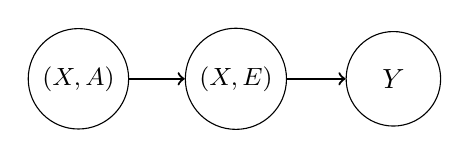
\begin{tikzpicture}

\node[circle,draw, minimum size=1.2cm] (R0) at (0,0) {\begin{small}$(X, A)$\end{small}
};
\node[circle,draw, minimum size=1.2cm] (R1) at (2,0) {\begin{small}$(X, E)$\end{small}};
\node[circle,draw, minimum size=1.2cm] (Y) at (4,0) {$Y$};

\path[->, thick] (R0) edge (R1);
\path[->, thick] (R1) edge (Y);

\end{tikzpicture}
\caption{Bayesian network corresponding to Assumption \ref{assum:indep-mips}.}
\label{fig:embedding_mips}
\vspace{-0.2cm}
% \end{wrapfigure}
\end{figure}


\myparagraph{Intuition}
The context-embedding pair $(X, E)$ can be seen as a representation of the context-action pair $(X, A)$ which contains less `redundant information' regarding the outcome $Y$. Intuitively, the MIPS estimator, which only considers the shift in the distribution of $(X, E)$ is therefore more efficient than the IPW estimator (which considers the shift in the distribution of $(X, A)$ instead). 
% In fact, as the representation $(X, E)$ gets closer to the outcome $Y$ in terms of information content, the variance of the MIPS estimator decreases. We formalise this in Appendix \faaiz{ref}. 

\myparagraph{MR achieves lower variance than MIPS}
Given the intuition above, we should achieve greater variance reduction as the amount of redundant information in the representation $(X, E)$ decreases. We formalise this in Appendix \ref{app:gmips} and show that the variance of MIPS estimator decreases as the representation gets closer to $Y$ in terms of information content. As a result, we achieve the greatest variance reduction by considering the marginal shift in the outcome $Y$ itself (as in MR) rather than the shift in the representation $(X, E)$ (as in MIPS). The following result formalizes this finding. 
% \jef{Ask Arnaud and Rob}
% As such, the greatest variance reduction is achieved when instead of considering the shift in the representation $(X, E)$ as in MIPS, we consider the marginal shift in the outcome $Y$ itself as in the MR estimator. The following results formalises this:
\begin{theorem}\label{prop:mips_main_text}
    When the weights $w(y)$, $\frac{\ptar(e, x)}{\pbeh(e, x)}$ and $\rho(a, x)$ are known exactly, then under Assumption \ref{assum:indep-mips}, 
    \begin{align*}
        \Ebeh[\thetamr] = \Ebeh[\hat{\theta}_{\textup{MIPS}}] = \Etar[Y], \quad \textup{and} \quad \Vbeh[\thetamr] \leq \Vbeh[\hat{\theta}_{\textup{MIPS}}] \leq \Vbeh[\thetaipw].
    \end{align*}
    % \[
    % \Vbeh[\thetamr] \leq \Vbeh[\hat{\theta}_{\textup{MIPS}}] \leq \Vbeh[\thetaipw].
    % \]
\end{theorem}
% \paragraph{Intuition}
This analysis provides a link between the MR and MIPS estimators in the framework of contextual bandits, and shows that the MR estimator achieves lower variance than MIPS estimator while not requiring any additional assumptions (e.g.\ Assumption \ref{assum:indep-mips} as in MIPS). We also verify this empirically in Section \ref{sec:exp-synth} by reproducing the experimental setup in \cite{saito2022off} along with the MR baseline.
% Proposition \ref{prop:mips_main_text} provides us an alternative perspective of the MR estimator. Both, the MIPS and the MR estimators lead to variance reduction by considering a representation of the context-action pair $(X, A)$ which contains less redundant information. However, in the case of the MR estimator, the representation under consideration is the outcome $Y$ itself and therefore it contains precisely the least amount of information necessary to obtain the outcome $Y$. Consequently, the variance of MR estimator is . Additionally, unlike the MIPS estimator, the MR estimator does not require any additional conditional independence assumptions.

% we replace the representation $(X, E)$ by the outcome $Y$ itself. In fact, this recovers the MR estimator.

% In fact, if instead of considering representations of 

% The intuitive reason behind the variance reduction is that the MIPS estimator considers the shift in the joint distribution of $(X, E)$ resulting from the policy shift.

\subsubsection{Weight estimation error}\label{subsec:weight-estimation-error}
% So far our analysis assumes that the behaviour policy $\beh$ and the marginal ratios $w(y)$ are known. However, in practice, both quantities may be unknown and must be estimated from data. To do so, we first split the available logged data $\D$ into training data $\Dtr = \{(x^\tr_i, a^\tr_i, y^\tr_i)\}_{i=1}^m$, which is used for weight estimation, and evaluation data $\Dev = \{(x_i, a_i, y_i)\}_{i=1}^n$, which is used to compute the OPE estimate. 
% % We then estimate the weights $w(y)$ using $\Dtr$ as follows:
% The estimation of weights $w(y)$ involves a two-step process, exclusively utilizing data from $\Dtr$ in each step:
Our analysis so far assumes prior knowledge of the behavior policy $\beh$ and the marginal ratios $w(y)$. However, in practice, both quantities are often unknown and must be estimated from data. To this end, we assume access to an additional training dataset $\Dtr = \{(x^\tr_i, a^\tr_i, y^\tr_i)\}_{i=1}^m$ (for weight estimation), in addition to the evaluation dataset $\D = \{(x_i, a_i, y_i)\}_{i=1}^n$ (for computing the OPE estimate). 
% More generally, these datasets can be obtained by splitting the available logged data.
% we first split the available logged data $\D$ into two subsets: the training data $\Dtr = \{(x^\tr_i, a^\tr_i, y^\tr_i)\}_{i=1}^m$ for weight estimation, and the evaluation data $\Dev = \{(x_i, a_i, y_i)\}_{i=1}^n$ for computing the OPE estimate.
The estimation of $\hat{w}(y)$ involves a two-step process that exclusively utilizes data from $\Dtr$:
% The weights $w(y)$ are then estimated using $\Dtr$ as follows:
% In practice, often the behaviour policy $\beh$ is not known and must be estimated through the logged observational data. 
\begin{enumerate}[label=(\roman*)]
    \item First, we estimate the policy ratio $\hat{\rho}(a, x) \approx \frac{\tar(a | x)}{\beh(a | x)}$. This can be achieved by estimating the behaviour policy $\hatbeh$, and defining $\hat{\rho}(a, x)\coloneqq \frac{\tar(a\mid x)}{\hatbeh(a\mid x)}$. Alternatively, $\hat{\rho}(a, x)$ can also be estimated directly by using density ratio estimation techniques as in \cite{sondhi2020balanced}.
    \item Secondly, we estimate the weights $\hat{w}(y)$ using Eq. \eqref{eq:weights-obj} with $\hat{\rho}$ instead of $\rho$.
\end{enumerate}

    % First, we estimate the behaviour policy $\hatbeh$, and define the policy ratio 
    % $
    % \hat{\rho}(A, X)\coloneqq \frac{\tar(a\mid x)}{\hatbeh(a\mid x)}.$
    % and use it to define the estimated ratios $\hat{\rho}(a, x)\coloneqq \tar(a\mid x)/\hatbeh(a\mid x)$.
 
% In this case, the policy ratio $\rho(a, x)$ is not known, and we resort to the use of estimated ratios $\hat{\rho}(a, x)\coloneqq \tar(a\mid x)/\hatbeh(a\mid x)$ instead.
% % This means the policy ratio $\rho(a, x)$ is not known, and must be estimated using the estimated behaviour policy, i.e.\ $\hat{\rho}(a, x)\coloneqq \tar(a\mid x)/\hatbeh(a\mid x)$. 
% The use of this ratio estimate $\hat{\rho}(a, x)$ may introduce bias in the IPW estimator. This also means that we have to rely on the estimated policy $\hatbeh$ to estimate the marginal ratio $w(y)$, which may also introduce a bias in the MR estimator. 

In practice, one may consider splitting $\Dtr$ for each estimation step outlined above. Moreover,
each approximation step may introduce bias and therefore, the MR estimator may have two sources of bias.
% the MR estimator may have two sources of bias: estimation of the behaviour policy $\hatbeh$, and the estimation of weights $\hat{w}(y)$.
% $$
% \hat{w}(y) \approx \Ebeh[\hat{\rho}(A, X)\mid Y=y] \qquad \textup{where, } \qquad  \hat{\rho}(a, x) \coloneqq \frac{\tar(a\mid x)}{\hatbeh(a\mid x)}.
% $$
While classical OPE methods like IPW and DR also suffer from bias because of $\hat{\rho}$ estimation, the estimation of $\hat{w}(y)$ is specific to MR. However, we show below
that given any policy ratio estimate $\hat{\rho}$, if $\hat{w}(y)$ approximates $\Ebeh[\hat{\rho}(A, X)\mid Y=y]$ `well enough' (i.e., the estimation step (ii) shown above is `accurate enough'), 
then MR achieves a lower variance than IPW and incurs little extra bias.

\begin{proposition}\label{prop:bias-and-var-main}
Suppose that the IPW and MR estimators are defined as,
\[
\approxipw \coloneqq \frac{1}{n}\sum_{i=1}^n\hat{\rho}(a_i, x_i)\, y_i, \quad \textup{and }\quad \approxmr \coloneqq \frac{1}{n}\sum_{i=1}^n\hat{w}(y_i)\, y_i,
\]
and define the approximation error as $\epsilon \coloneqq \hat{w}(Y) - \tilde{w}(Y)$, where $\tilde{w}(Y) \coloneqq \Ebeh[\hat{\rho}(A, X)\mid Y]$. Then we have that, $\textup{Bias}(\approxmr) - \textup{Bias}(\approxipw) = \Ebeh[\epsilon\,Y]$. Moreover,
% $\Ebeh[\epsilon] = 0$ and 
% $\epsilon \indep Y$. Then, 
% \begin{align*}
%     \textup{Bias}(\thetamr) &= \textup{Bias}(\thetaipw) \quad \textup{and,} \\
%     n (\Vbeh[\thetaipw] - \Vbeh[\thetamr]) 
%     &= \E_{Y\sim \pbeh(Y)} \left[ \Vbeh\left[ \hat{\rho}(A, X) \mid Y \right]\, Y^2 \right] - \Vbeh[\epsilon]\,\Ebeh[Y^2].
% \end{align*}
\begin{small}
\begin{align}
    \Vbeh[\approxipw] - \Vbeh[\approxmr]
    % &= \frac{1}{n}\left(\underbrace{\Ebeh[\Vbeh[\hat{\rho}(A, X)\,Y\mid Y]]}_{\geq 0} - \Vbeh[\epsilon\,Y] - 2\,\textup{Cov}(\tilde{w}(Y)\,Y, \epsilon\,Y)\right). \label{eq:var-difference-approximate-weights}
    &= \frac{1}{n}(\underbrace{\Ebeh[\Vbeh[\hat{\rho}(A, X)\,Y\mid Y]]}_{\geq 0} - \Vbeh[\epsilon\,Y] - 2\,\textup{Cov}(\tilde{w}(Y)\,Y, \epsilon\,Y)). \label{eq:var-difference-approximate-weights}
\end{align}
\end{small}
% and,
% \begin{align*}
%     &n (\Vbeh[\approxipw] - \Vbeh[\approxmr]) \\
%     &\quad= \Ebeh[\Vbeh[\hat{\rho}(A, X)\mid Y]\,Y^2] - \Vbeh[\epsilon\,Y] - 2\,\textup{Cov}(\Ebeh[\hat{\rho}(A, X)\mid Y]\,Y, \epsilon\,Y).
% \end{align*}
\end{proposition}
% if $\Ebeh[\hat{\rho}(A, X)\mid Y]$ is estimated `well enough', MR achieves a lower variance than IPW and does not incur any extra bias compared to IPW.
\myparagraph{Intuition} The $\epsilon$ term defined in Proposition \ref{prop:bias-and-var-main} denotes the error of the second approximation step outlined above. 
As a direct consequence of this result, we show in Appendix \ref{sec:wide_nns_weight_estimation} that as the error $\epsilon$ becomes small (specifically as $\Ebeh[\epsilon^2]\rightarrow 0$), the difference between biases of MR and IPW estimator becomes negligible.
% The result shows that as the error $\epsilon$ becomes small, i.e. $\epsilon \overset{\textup{a.s.}}{\rightarrow}0$, the difference between biases of MR and IPW estimator decreases. 
Likewise, the terms $\Vbeh[\epsilon\,Y]$ and $\textup{Cov}(\tilde{w}(Y)\,Y, \epsilon\,Y)$ in Eq. \eqref{eq:var-difference-approximate-weights} will also be small and as a result the variance of MR will be lower than that of IPW (as the first term is positive). 

In fact, using recent results regarding the generalisation error of neural networks \citep{lai2023generalization}, we show that when using 2-layer wide neural networks to approximate the weights $\hat{w}(y)$, the estimation error $\epsilon$ declines with increasing training data size $m$. Specifically, under certain regularity assumptions we obtain $\Ebeh[\epsilon^2] = O(m^{-2/3})$. Using this we show that as the training data size $m$ increases, the biases of MR and IPW estimators become roughly equal with a high probability, and
\[
\Vbeh[\approxipw] - \Vbeh[\approxmr] = \frac{1}{n}\,\Ebeh[\Vbeh[\hat{\rho}(A, X)\,Y\mid Y]] + O(m^{-1/3}).
\]
Therefore the variance of MR estimator falls below that of IPW for large enough $m$. The empirical results shown in Appendix \ref{subsec:mips-empirical} are consistent with this result. Due to space constraints, the main technical result has been included in Appendix \ref{sec:wide_nns_weight_estimation}.

% number of training samples $m$ increases, the biases of MR and IPW estimators become roughly equal, whereas the variance of MR estimator falls below that of the IPW estimator. The empirical results shown in Appendix \ref{subsec:additional-experiments} are consistent with this result.
% Moreover, in Theorem \ref{prop:informal}, the estimated policy ratio $\hat{\rho}(a, x)$ is fixed for increasing $m$, i.e., we do not update $\hat{\rho}(a, x)$ as more training data becomes available. While this may seem as a disadvantage for the IPW estimator, we point out that the result also holds when the policy ratio is exact (i.e., $\hat{\rho}(a, x) = \rho(a, x)$) and hence the IPW estimator is unbiased.

% In fact, using recent results regarding the generalisation error of wide neural networks \citep{lai2023generalization}, we can show that when using 2-layer wide neural networks to approximate the weights $\hat{w}(y)$, the estimation error of the second approximation step above scales as $O(m^{-1/3})$ where $m$ is the number of training data used to approximate $\hat{w}(y)$.
% % Using recent results regarding the generalisation error of wide neural networks \citep{lai2023generalization}, we show that when using 2-layer wide neural networks to approximate the weights $\hat{w}(y)$, then under mild assumptions, $\Ebeh[\epsilon^2]\leq O(m^{-2/3})$. Here $m$ is the number of training data used to approximate $\hat{w}(y)$. 
% Due to space constraints, we include an informal statement of the result here. The main technical result has been included in Appendix \ref{sec:wide_nns_weight_estimation}.

% \begin{theorem}[Informal Statement]\label{prop:informal}
% % Let $\mathcal{D}_{tr}$ be training data with $m$ samples $\{(x^\tr_i, a^\tr_i, y^\tr_i)\}_{i=1}^m$.
% Suppose that the IPW and MR estimators are defined as,
% \[
% \approxipw \coloneqq \frac{1}{n}\sum_{i=1}^n\hat{\rho}(a_i, x_i)\, y_i, \quad \textup{and }\quad \approxmr \coloneqq \frac{1}{n}\sum_{i=1}^n\hat{w}(y_i)\, y_i,
% \]
% % and let
% % \[
% % \thetamr = \frac{1}{n}\sum_{i=1}^n\hat{w}(y_i)\, y_i,
% % \]
% where $\hat{w}(y)$ is approximated by minimising the following empirical loss on a training dataset of size $m$, $\mathcal{D}_{tr}\coloneqq \{(x^\tr_i, a^\tr_i, y^\tr_i)\}_{i=1}^m$ (disjoint from evaluation dataset $\{(x_i, a_i, y_i)\}_{i=1}^n$):
% % \[
% %     \mathcal{L}(\theta) = \E_{\mathcal{D}_{tr}}(\hat{\rho}(A, X) - f_\phi(Y))^2.
% % \]
% \[
%     \mathcal{L}(\phi) = \E_{(X, A, Y)\sim \mathcal{D}_{tr}} \left[\left(\hat{\rho}(A, X) - f_{\phi}(Y)\right)^2\right].
% \]
% If $f_\phi$ is a two-layer neural network with large enough width and for sufficiently large $m$, then under the regularity assumptions provided in Appendix \ref{sec:wide_nns_weight_estimation}, the following holds with high probability,
% \begin{align*}
%     |\textup{Bias}(\approxmr) - \textup{Bias}(\approxipw)| &= O(m^{-1/3}),\\
%     \Vbeh[\approxipw] - \Vbeh[\approxmr] &= \frac{1}{n}\underbrace{\Ebeh[\Vbeh[\hat{\rho}(A, X)\mid Y]\, Y^2]}_{\geq 0} + O(m^{-2/3}).
% \end{align*}
% % holds with high probability. 
% \end{theorem}

% \myparagraph{Intuition} This theorem shows that as the number of training samples $m$ increases, the biases of MR and IPW estimators become roughly equal, whereas the variance of MR estimator falls below that of the IPW estimator. The empirical results shown in Appendix \ref{subsec:additional-experiments} are consistent with this result.
% Moreover, in Theorem \ref{prop:informal}, the estimated policy ratio $\hat{\rho}(a, x)$ is fixed for increasing $m$, i.e., we do not update $\hat{\rho}(a, x)$ as more training data becomes available. While this may seem as a disadvantage for the IPW estimator, we point out that the result also holds when the policy ratio is exact (i.e., $\hat{\rho}(a, x) = \rho(a, x)$) and hence the IPW estimator is unbiased.
 
% In this section, we show that under certain assumptions, the use of the estimated importance weights $\hat{w}(y)$ rather than $\hat{\rho}(a, x)$ does not worsen the bias of the resulting OPE estimator. Moreover, if $\hat{w}(y)$ are estimated `well enough', the variance of MR estimator will be lower than that of IPW estimator in this case as well. The following result formalises this:
% \begin{align}
%     \hat{w} = \arg\min_{f} \, \Ebeh \Bigg[\frac{\tar(A|X)}{\hatbeh (A|X)}-f(Y)\Bigg]^2, \label{eq:estimated-marginal-ratio}
% \end{align}
% then the bias in the MR estimator will be equal to the bias in the IPW estimator. This means that in the case when $\beh$ is approximated and the marginal ratio estimate $\hat{w}(y)$ are obtained by exactly regressing to the approximate policy ratios $\hat{\rho}(a, x)$, the biases of the MR and IPW estimators will be identical. Additionally, the result in Proposition \ref{prop:var_mr} straightforwardly extends to this case, showing that if the marginal ratios $\hat{w}(y)$ are estimated `well enough', the variance of MR estimator will be lower than that of IPW estimator in this case as well.

\subsection{Application to causal inference}\label{subsec:application-to-causal-inference}
 Beyond contextual bandits, the variance reduction properties of the MR estimator make it highly useful in a wide variety of other applications. Here, we show one such application in the field of causal inference, where MR can be used for the estimation of average treatment effect (ATE) \citep{pearl2009causality} and leads to some desirable properties in comparison to the conventional ATE estimation approaches. Specifically, we illustrate that the MR estimator for ATE utilizes the evaluation data $\D$ more efficiently and achieves lower variance than state-of-the-art ATE estimators and consequently provides more accurate ATE estimates.
% leads to a significantly more data efficient methodology with  
% This comparative advantage of MR becomes even more apparent when the observational data size is small.
% We show, both theoretically and empirically, that our methodology provides more reliable ATE estimation overall, and performs especially better than other baselines when the number of data is low.
% The MR estimator can also be applied in the setting of causal inference for estimation of average treatment effect (ATE) and leads to more data efficient methodology than many state-of-the-art ATE estimators.
To be concrete, the goal in this setting is to estimate ATE, defined as follows:
% Off-Policy evaluation is widely applied sin causal inference, where often the goal is to estimate the average treatment effect (ATE), defined as follows:
\[
\ate \coloneqq \E[Y(1)-Y(0)].
\]
Here $Y(a)$ corresponds to the outcome under a deterministic policy $\pi_a(a'\mid x) \coloneqq \ind(a'=a)$. Hence any OPE estimator can be used to estimate $\E[Y(a)]$ (and therefore ATE) by considering target policy $\tar = \pi_a$.
% Given an OPE estimator, $\E[Y(a)]$ 
% We can use any OPE estimator with deterministic target policies to estimate the ATE. 
% We provide explicit expressions of ATE estimators using MR, IPW and DR in Appendix \ref{app:causal-inference}.
An important distinction between MR and existing approaches (like IPW or DR) is that, when estimating $\E[Y(a)]$, the existing approaches only use datapoints in $\D$ with $A=a$. To see why this is the case, we note that the policy ratios $\frac{\tar(A|X)}{\beh(A|X)} = \frac{\ind(A=a)}{\beh(A|X)}$ are zero when $A\neq a$. In contrast, the MR weights $\frac{\ptar(Y)}{\pbeh(Y)}$ are not necessarily zero for datapoints with $A\neq a$, and therefore the MR estimator uses all evaluation datapoints when estimating $\E[Y(a)]$. 

As such we show that MR applied to ATE estimation leads to a smaller variance than the existing approaches. Moreover, because MR is able to use all datapoints when estimating $\E[Y(a)]$, MR will generally be more accurate than the existing methods especially in the setting where the data is imbalanced, i.e., the number of datapoints with $A=a$ is small for a specific action $a$.
In Appendix \ref{app:causal-inference}, we formalise this variance reduction of the MR ATE estimator compared to IPW and DR estimators, by deriving analogous results to Propositions \ref{prop:var_mr} and \ref{prop:var_dr}. In addition, we also show empirically in Section \ref{subsec:causal-experiments} that the MR ATE estimator outperforms the most commonly used ATE estimators.
\begin{comment}

\begin{proposition}\label{prop:bias-and-var}
Let 
\[
\thetaipw = \frac{1}{n}\hat{\rho}(a_i, x_i)\, y_i,
\]
where $\hat{\rho}(a, x)\coloneqq \tar(a\mid x)/\hatbeh(a\mid x)$. Additionally, let
\[
\thetamr = \frac{1}{n}\hat{w}(y_i)\, y_i,
\]
where $\hat{w}(y)$ satisfies Eq. $\eqref{eq:estimated-marginal-ratio}$. Then, 
\begin{align*}
    \textup{Bias}(\thetamr) &= \textup{Bias}(\thetaipw) \qquad \textup{and,} \\
    n (\Vbeh[\thetaipw] - \Vbeh[\thetamr]) 
    &= \E_{Y\sim \pbeh(Y)} \left[ \Vbeh\left[ \hat{\rho}(A, X) \mid Y \right]\, Y^2 \right].
\end{align*}
\end{proposition}
More generally, if $\hat{w}$ is a `noisy' estimate of the conditional expectation $\Ebeh[\hat{\rho}(A, X)\mid Y]$, we can obtain similar results regarding the bias and variance of the MR estimators under certain assumptions. 
\end{comment}


% Using recent results regarding the generalisation error of wide neural networks \citep{lai2023generalization}, we show that when using 2-layer wide neural networks to approximate the weights $\hat{w}(y)$, then under mild assumptions, $\Ebeh[\epsilon^2]\leq O(m^{-2/3})$. Here $m$ is the number of training data used to approximate $\hat{w}(y)$. Due to space constraints, we include an informal statement of the result here. The main technical result has been included in Appendix \ref{sec:wide_nns_weight_estimation}.

% Additionally, replacing the true behaviour policy $\beh$ by the estimate $\hatbeh$ in Eq. \eqref{eq:weights-obj} will 

% if we approximate the marginal ratio $w(y)$ using the approximate 



\begin{comment}
    

Specifically, the traditional IPW estimator applied to ATE estimation yields:
\[
\ateipw = \frac{1}{n} \sum_{i=1}^n \rho_{\ate}(a_i, x_i) \times y_i, \qquad \textup{where, } \qquad \rho_{\ate}(a, x) \coloneqq \frac{\mathbbm{1}(a=1) - \mathbbm{1}(a=0)}{\beh (a|x)}.
\]

Simlarly, the MR estimator can be written as
$$
\atemr = \frac{1}{n}\sum_{i=1}^n w_{\ate}(y_i)\times y_i, \qquad \textup{where, } \qquad w_{\ate}(y) = \frac{p_{\pi^{(1)}}(y) - p_{\pi^{(0)}}(y)}{\pbeh(y)},
$$ 
and $\pi^{(a)}(a'\mid x) \coloneqq \mathbbm{1}(a'=a)$ for $a\in \{0,1\}$, and $w_{\ate}(y)$ can be estimated using regression similar to Eq. \eqref{eq:weights-obj}.
\end{comment}
% Again, using the fact that $w_{\ate}(Y) \eqas \E[\rho_{\ate}(A, X)\mid Y]$, we can obtain $w_{\ate}$ by minimising a simple mean-squared loss:
% \begin{align*}
%     w_{\ate} =\arg \min_{f} \Ebeh \Big[\frac{\mathbbm{1}(A=1)- \mathbbm{1}(A=0)}{\beh (A|X)}-f(Y)\Big]^2
% \end{align*}

% For the MR estimator, we don't need to estimate weights for $Y(1)$ and $Y(0)$ separately, as we can combine the two as follows:
% \begin{align}
%     w_{\ate} =\arg \min_{f} \Ebeh \Big[\frac{\mathbbm{1}(A=1)- \mathbbm{1}(A=0)}{\beh (A|X)}-f(Y)\Big]^2 \label{eq:ate-weights-loss}
% \end{align}
% It follows straightforwardly from Lemma \ref{prop:weights-est}, that the function that minimises  \eqref{eq:ate-weights-loss} is equal to 
% \[
% w_{\ate}(y) = \frac{p_{\pi^{(1)}}(y) - p_{\pi^{(0)}}(y)}{\pbeh(y)},
% \] 
% where $\pi^{(a)}(a'\mid x) \coloneqq \mathbbm{1}(a'=a)$ for $a\in \{0,1\}$.
% Then, the MR estimator can be written as
% $$\atemr = \frac{1}{n}\sum_{i=1}^n w_{\ate}(y_i)\times y_i.$$ 
% In contrast, the traditional IPW estimator is of the form:
% \[
% \ateipw = \frac{1}{n} \sum_{i=1}^n \rho_{\ate}(a_i, x_i) \times y_i,
% \]
% where 
% \[
% \rho_{\ate}(a, x) \coloneqq \frac{\mathbbm{1}(a=1) - \mathbbm{1}(a=0)}{\beh (a|x)}.
% \]

\section{Related Work}
Off-Policy evaluation is a central problem both in contextual bandits \citep{dudik2014doubly, wang2017optimal, liu2018breaking, farajtabar2018more, su2019continuous, su2020doubly, kallus2021optimal, metelli2021subgaussian, saito2020open} and in RL \citep{thomas2016data, xie2019advances, kallus2020off, liu2020understanding}. 
Existing OPE methodologies can be broadly categorised into Direct Method (DM), Inverse Probability Weighting (IPW), and Doubly Robust (DR). 
While DM typically has a low variance, it suffers from high bias when the reward model is misspecified \citep{voloshin2021empirical}. 
On the other hand, IPW \citep{horvitz1952generalization} and DR \citep{dudik2014doubly, wang2017optimal, su2020doubly} use policy ratios as importance weights when estimating policy value and suffer from high variance as overlap between behaviour and target policies increases or as the action/context space gets larger \citep{sachdeva2020off, saito2022off}. To circumvent this problem, techniques like weight clipping or normalisation \citep{swaminathan2015counterfactual, swaminathan2015the, chaudhuri2019london} are often employed, however, these can often increase bias.

% The IPW estimator \citep{horvitz1952generalization} can have low bias but suffers from high variance as overlap between behaviour and target policies increases or as the action/context space gets larger \citep{sachdeva2020off, saito2022off}. To circumvent this problem, techniques like weight clipping or normalisation \citep{swaminathan2015counterfactual, swaminathan2015the} are often employed, however, these can often lead to the worsening of bias.



% The second class of methodologies, called the Inverse Probability Weighting (IPW) \citep{horvitz1952generalization}, uses importance weights to estimate the value of the target policy. If the behaviour policy is well-estimated, the IPW estimator will have a low bias. However, IPW can suffer from a high variance especially as the overlap between behaviour and target policies increases, or as the size of action and/or context space increases \citep{sachdeva2020off}. To circumvent this problem, techniques like weight clipping or normalisation \citep{swaminathan2015counterfactual, swaminathan2015the} are often employed, however, these can often lead to the worsening of bias. 

% The DR method \citep{dudik2014doubly} and its extensions \citep{wang2017optimal, su2020doubly} combine the direct method with importance sampling and achieves better overall bias and variance than the IPW method. However, like the IPW method these DR methods also take the shift of joint distributions of $(X, A, Y)$ into consideration when estimating policy value. As we show in Section \ref{subsec:comparison}, this can lead to high variance especially as the policy shift increases or the action and/or context space gets larger. 

In contrast to these approaches, \cite{saito2022off} propose MIPS, which considers the marginal shift in the distribution of a lower dimensional embedding of the action space. While this approach reduces the variance associated with IPW, we show in Section \ref{subsec:mips-comparison} that the MR estimator achieves a lower variance than MIPS while not requiring any additional assumptions (like Assumption \ref{assum:indep-mips}).
% it requires conditional independence assumptions on the embedding $R$, the violation of which may lead to high bias. 
% We show in Section \ref{subsec:mips-comparison} that in comparison, the MR estimator does not require any such conditional independence assumptions, and achieves a lower variance than the MIPS estimator by only considering the shift in the marginal distribution of the reward $Y$. 

In the context of Reinforcement Learning (RL), various marginalisation techniques of importance weights have been used to propose OPE methodologies.
% OPE methodologies using marginalised importance weighting have been proposed 
% \citep{liu2018breaking, xie2019advances, Fujimoto2021deep, rowland2020conditional}
% \citep{thomas2016data, xie2019advances, kallus2020off, liu2020understanding}. 
\cite{liu2018breaking, xie2019advances, kallus2020off} use methods which considers the shift in the marginal distribution of the states, and applies importance weighting with respect to this marginal shift rather than the trajectory distribution. Similarly, \cite{Fujimoto2021deep} use marginalisation for OPE in deep RL, where the goal is to consider the shift in marginal distributions of state and action. Although marginalization is a key trick of these estimators, these techniques do not consider the marginal shift in reward as in MR and are aimed at resolving the curse of horizon, a problem specific to RL. Apart from this, \cite{rowland2020conditional} propose a general framework of OPE based on conditional expectations of importance ratios for variance reduction. While their proposed framework includes reward conditioned importance ratios, this is not the main focus and there is little theoretical and empirical comparison of their proposed methodology with existing state-of-the-art methods like DR. 

Finally we note that the idea of approximating the ratio of intractable marginal densities via leveraging the fact that this ratio can be reformulated as the conditional expectation of a ratio of tractable densities is a standard idea in computational statistics \cite{meng1996simulating} and has been exploited more recently to perform likelihood-free inference \cite{brehmer2020mining}. In particular, while  \cite{meng1996simulating} typically approximates this expectation through Markov chain Monte Carlo, \cite{brehmer2020mining} uses regression instead, however without any theory.
% of this approach has been carried out in \cite{brehmer2020mining}.

% Our work introduces the marginal ratio estimator for OPE in contextual bandits. We provide extensive theoretical and empirical comparisons of our proposed estimator with existing methods, and show that the MR estimator performs especially better than the other methods in large actions and/or context spaces. 
% \faaiz{@Arnaud and Rob: what are your thoughts about this characterisation of \cite{rowland2020conditional}?}

% Our work proposes an OPE methodology for contextual bandits which only considers the shift in the marginal distribution of rewards. In addition, we include extensive theoretical and empirical comparisons of our proposed estimator with existing methods, and show that the MR estimator performs especially better than the other methods in large actions and/or context spaces. 

\begin{comment}
\begin{itemize}
    \item IPW
    \item Double robust methods
    \item Debiased methods 
    \item See related works in \cite{saito2022off}
\end{itemize}
\subsection{Baselines in Contextual Bandits setting}
\begin{itemize}
    \item \cite{thomas2016data, saito2021evaluating, saito2022off,wang2017optimal}
    \item Using ideas from \cite{saito2022off},  we can show that our methodology requires common support of $\pbeh(Y\mid X)$ and $\ptar(Y\mid X)$ which is weaker than requiring common supports of $\beh(A\mid X)$ and $\tar(A\mid X)$, which is needed for IPW estimator. We can show that our estimator has a smaller variance than the methodology proposed by \cite{saito2022off}. Moreover, we should show empirically that, as a consequence of this, our estimator is more robust to heavy-tailed policy ratios. The baselines considered in this paper are the ones to compare against.
    \item \cite{wang2017optimal} proposes a SWITCH estimator for policy evaluation, and show that this estimator is minimax optimal when the hyperparameter $\tau$ is chosen appropriately. Moreover, this estimator is more robust to large (or heavy-tailed) importance weights. It also includes an expression for the variance of the DR estimator which could be useful.
    \item \cite{saito2021evaluating}: In this work, the authors develop Interpretable Evaluation for Offline Evaluation (IEOE), an experimental procedure to evaluate OPE estimators’ robustness to changes in hyperparameters and/or evaluation policies in an interpretable manner. This is more of a review paper.
    \item \cite{liu2019triply}: Could be an interesting baseline. The background section of this paper seems interesting. 
\end{itemize}
\subsection{Marginalised Importance Sampling in Reinforcement Learning}
The main difference between this line of work and our idea is that these works consider the marginal distribution over the states. Instead, we propose considering the marginal distribution over rewards directly. 
\begin{itemize}
    \item \cite{liu2018breaking}: The paper originally proposed avoiding the long horizon problem by computing MIS over state distributions rather than entire trajectories. The marginal ratio in these works is different to ours.  
    \item \cite{Fujimoto2021deep}: Applies the MIS idea to deep RL setting: Marginalized importance sampling (MIS), which measures the density ratio between the state-action occupancy of a target policy and that of a sampling distribution, is a promising approach for off-policy evaluation. However, current state-of-the-art MIS methods rely on complex optimization tricks and succeed mostly on simple toy problems. This paper bridges the gap between MIS and deep reinforcement learning by observing that the density ratio can be computed from the successor representation of the target policy. 
    \item \cite{kallus2020off}: The related works section of this paper is very useful. In this work, the authors propose the use of a marginal importance sampling estimator which is somewhat similar to ours (although not the same). Would be useful to read this in depth.
    \item \cite{xie2019advances}: Avoiding the long horizon problem by computing IS over state distributions rather than trajectories - was already introduced in \cite{liu2018breaking}, which the authors cite sufficiently often in the text. However, the approach the authors take to leveraging this idea is original. The estimation technique for the ratios is also different -- the authors propose a recursive estimation technique to estimate the marginal distribution ratios over states. 
    \item \cite{liu2020understanding} also references MIS estimators. 
    \item \cite{rowland2020conditional}: This paper proposes conditional importance sampling for variance reduction in RL setting. The paper considers a general conditioning strategy, based on conditioning importance weights on different statistics. They also mention reward conditional importance sampling. \textbf{Important paper.} 
\end{itemize}
\end{comment}


\section{Empirical evaluation}
In this section, we provide empirical evidence to support our theoretical results by investigating the performance of our MR estimator against the current state-of-the-art OPE methods. The code to reproduce our experiments has been made available at: \href{https://github.com/faaizT/MR-OPE}{\textcolor{blue}{github.com/faaizT/MR-OPE}}.
% Here, we present a synthetic data experiment and also consider an application of MR to causal inference. 
% Additional experiments that support our proposed method MR on real-world classification datasets are provided in Appendix \ref{app:experiments} due to space constraints. \faaiz{Squeeze in classification exps in main}
% We first consider a synthetic setup to conduct extensive ablation study
% We evaluate MR estimator on synthetic data to identify the cases where it offers more accurate off-policy evaluation. These experiments are conducted using the \emph{OpenBanditPipeline} (OBP)
% % \footnote{\url{https://github.com/st-tech/zr-obp}}
% , an open-source package for OPE developed by \cite{saito2020open}.

\subsection{Experiments on synthetic data}\label{sec:exp-synth}
For our synthetic data experiment, we reproduce the experimental setup for the synthetic data experiment in \cite{saito2022off} by reusing their code with minor modifications.
% We use synthetically generated dataset for this experiment. 
Specifically, $\Xspace \subseteq \mathbb{R}^d$, for various values of $d$ as described below. Likewise, the action space $\Aspace = \{0, \dots, n_a-1\}$, with $n_a$ taking a range of different values. Additional details regarding the reward function, behaviour policy $\beh$, and the estimation of weights $\hat{w}(y)$ have been included in Appendix \ref{subsec:mips-empirical} for completeness. 

% $d$-dimensional context vectors $x$ are sampled from a standard normal distribution, i.e.\ $\Xspace \subseteq \mathbb{R}^d$, for various values of $d$ as described below. Likewise, the action space is finite and comprises of $n_a$ actions, i.e.\ $\Aspace = \{0, \dots, n_a-1\}$, with $n_a$ taking a range of different values. 
% Due to space constraints, we include additional details regarding the reward function, behaviour policy $\beh$, and the estimation of weights $\hat{w}(y)$ in Appendix \ref{sec:app-additional-results}. 


\myparagraph{Target policies} 
To investigate the effect of increasing policy shift, we define a class of policies,
\[
% \vspace{-0.05cm}
\pi^{\alpha^\ast}(a | x) = \alpha^\ast\,\ind(a = \arg\max_{a'\in \Aspace} q(x, a')) + \frac{1-\alpha^\ast}{|\Aspace|} \quad \textup{where} \quad q(x, a) \coloneqq \E[Y\mid X=x, A=a],
% \vspace{-0.05cm}
\]
where $\alpha^\ast \in [0, 1]$ allows us to control the shift between $\beh$ and $\tar$. In particular, as we show later, the shift between $\beh$ and $\tar$ increases as $\alpha^\ast \rightarrow 1$. Using the ground truth behaviour policy $\beh$, we generate a dataset which is split into training and evaluation datasets of sizes $m$ and $n$ respectively. 


% \paragraph{Reward function}
% The expected reward $q(x, a)\coloneqq\E[Y\mid x, a]$ for these experiments is defined as follows:
% \[
%     q(x, a) = \sin \left(a \cdot ||x||_2 \right). 
% \]
% The reward $Y$ is obtained by adding a normal noise random variable to $q(x, a)$
% \[
% Y = q(X, A) + \epsilon, 
% \]
% where $\epsilon \sim \mathcal{N}(0, 0.01)$.

% \paragraph{Behaviour and target policies}
% We first define a behaviour policy by applying softmax function to $q(x, a)$ as
% \[
% \beh(a\mid x) = \frac{\exp{(q(x, a))}}{\sum_{a' \in \Aspace} \exp{(q(x, a'))}}.
% \]

% where $\beta$ controls the optimality and entropy of the policy $\pi_\beta$. A large positive value of $\beta$ leads to a near-deterministic and well-performing policy, while lower values make the policy increasingly worse and `noisy'. 
% In this experiment, we define the behaviour policy as $\beh = \pi_{\beta^b}$ for $\beta^b = 0.5$ and target policies as $\tar= \pi_{\beta^\ast}$ for $\beta^\ast \in \{0.0, 0.5, 1.0, \ldots, 5.0 \}$.
% In contrast, for the target policy, we define the class of parametric policies,
% \[
% \pi^{\alpha^\ast}(a | x) = \alpha^\ast\,\ind(a = \arg\max_{a'\in \Aspace} q(x, a')) + \frac{1-\alpha^\ast}{|\Aspace|},
% \]
% where $\alpha^\ast \in [0, 1]$ controls the quality of $\pi^{\alpha^\ast}$. In particular, as $\alpha^\ast \rightarrow 1$, the target policy approaches the optimal policy. 


\myparagraph{Baselines} 
We compare our estimator with DM, IPW, DR and MIPS estimators. Our setup includes action embeddings $E$ satisfying Assumption \ref{assum:indep-mips}, and so MIPS is unbiased.
% Since there is no natural action embedding $E$ in our setup which satisfies Assumption \ref{assum:indep-mips}, we instead consider a generalised version of MIPS (defined as G-MIPS in Appendix \ref{app:gmips}) which uses an embedding of context-action pair $(X, A)$ rather than an embedding of the action $A$.
% \footnote{We also compare against the original MIPS estimator in Appendix \ref{subsec:mips-empirical} by reproducing the setup of \cite{saito2022off}}
Additional baselines have been considered in Appendix \ref{subsec:mips-empirical}.
For MR, we split the training data to estimate $\hatbeh$ and $\hat{w}(y)$, whereas for all other baselines we use the entire training data to estimate $\hatbeh$ for a fair comparison.
% In addition, we also consider Switch-DR \citep{wang2017optimal} and DR with Optimistic Shrinkage (DRos) \citep{su2020doubly}. 
% To estimate $\hat{q}(x, a)$ for DM and DR estimators, we use multi-layer perceptrons (MLPs). \jef{last sentence not needed}
% \jef{I personally think having the legend at the top is better as now it is asymetric ... not a big deal though lol (fig2)
% }
\begin{figure}[t]
     \centering
     \begin{subfigure}[b]{0.5\textwidth}
         \centering
         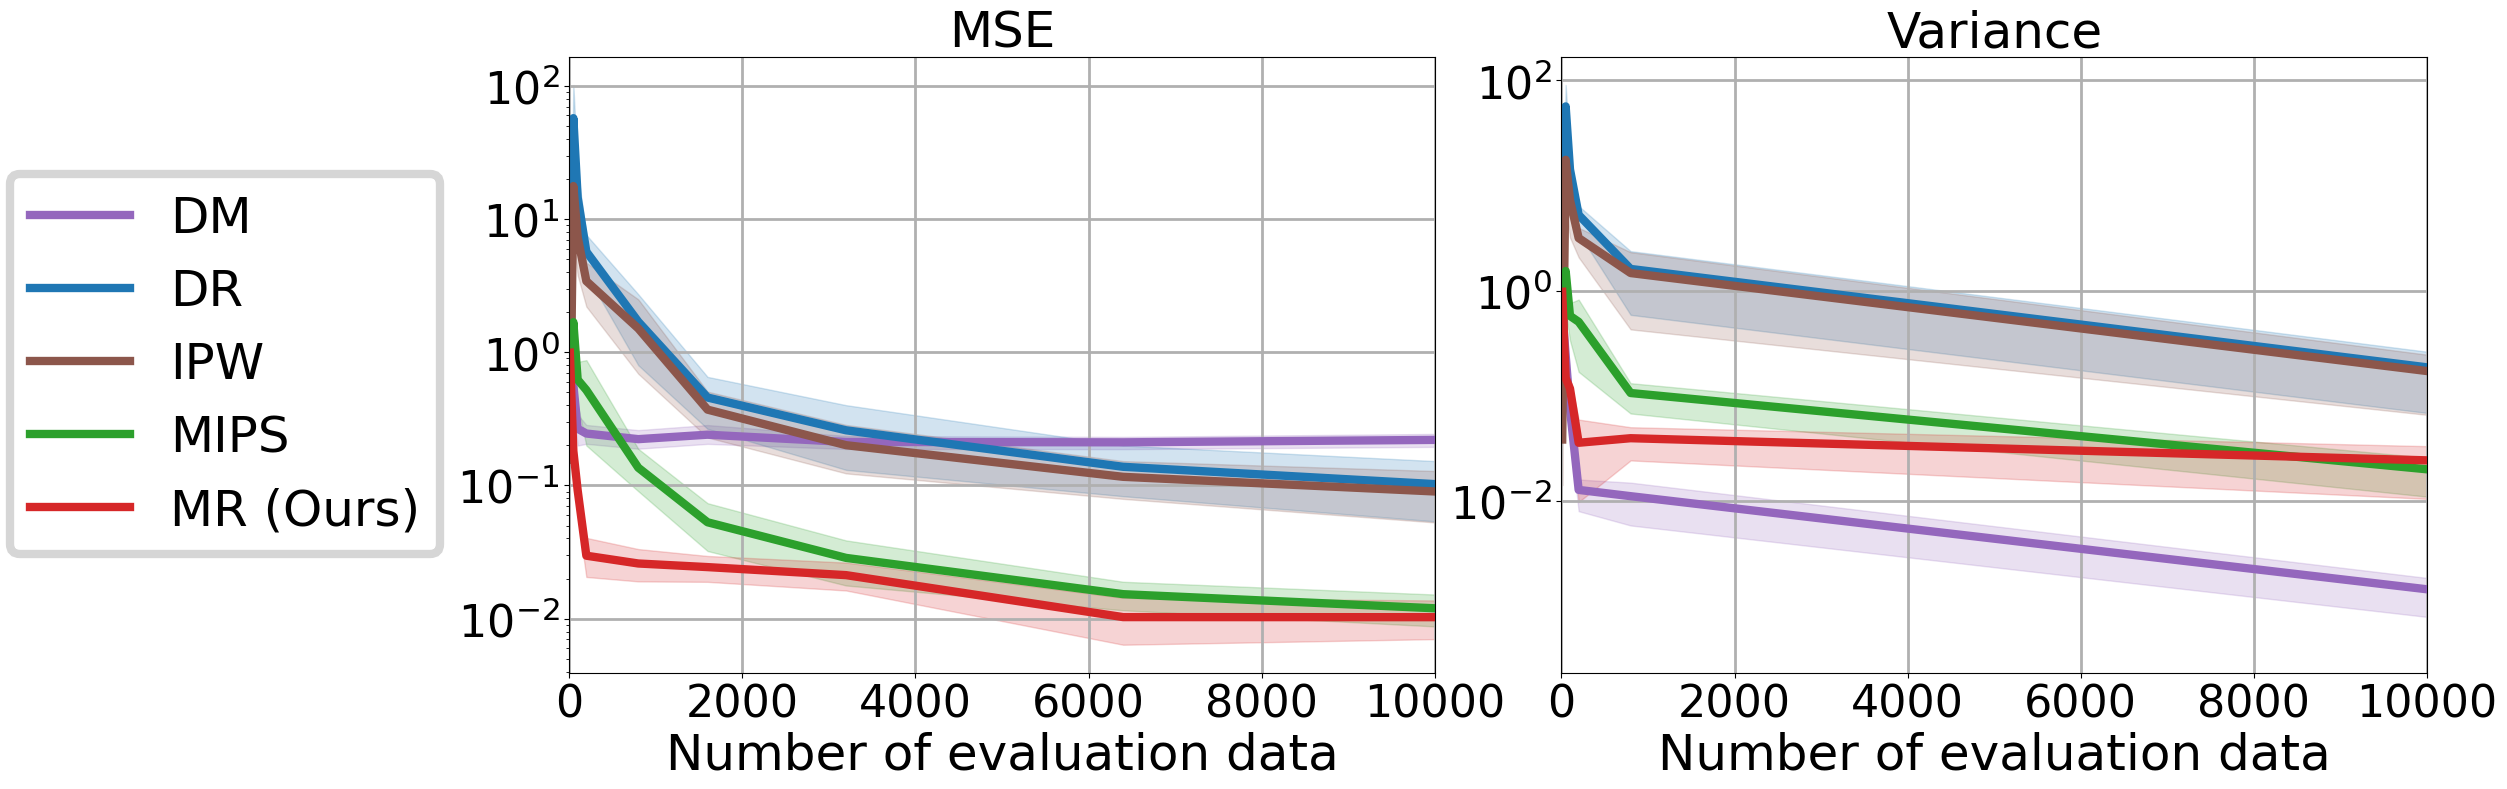
\includegraphics[height=1.06in]{figures/mr/ope_vs_neval_nac_100_alphatar_0_8_dimc_1000_untrunc.png}
         \caption{Results with varying evaluation data size $n$.}
         \label{fig:mse-vs-neval}
     \end{subfigure}%
     \begin{subfigure}[b]{0.5\textwidth}
         \centering
         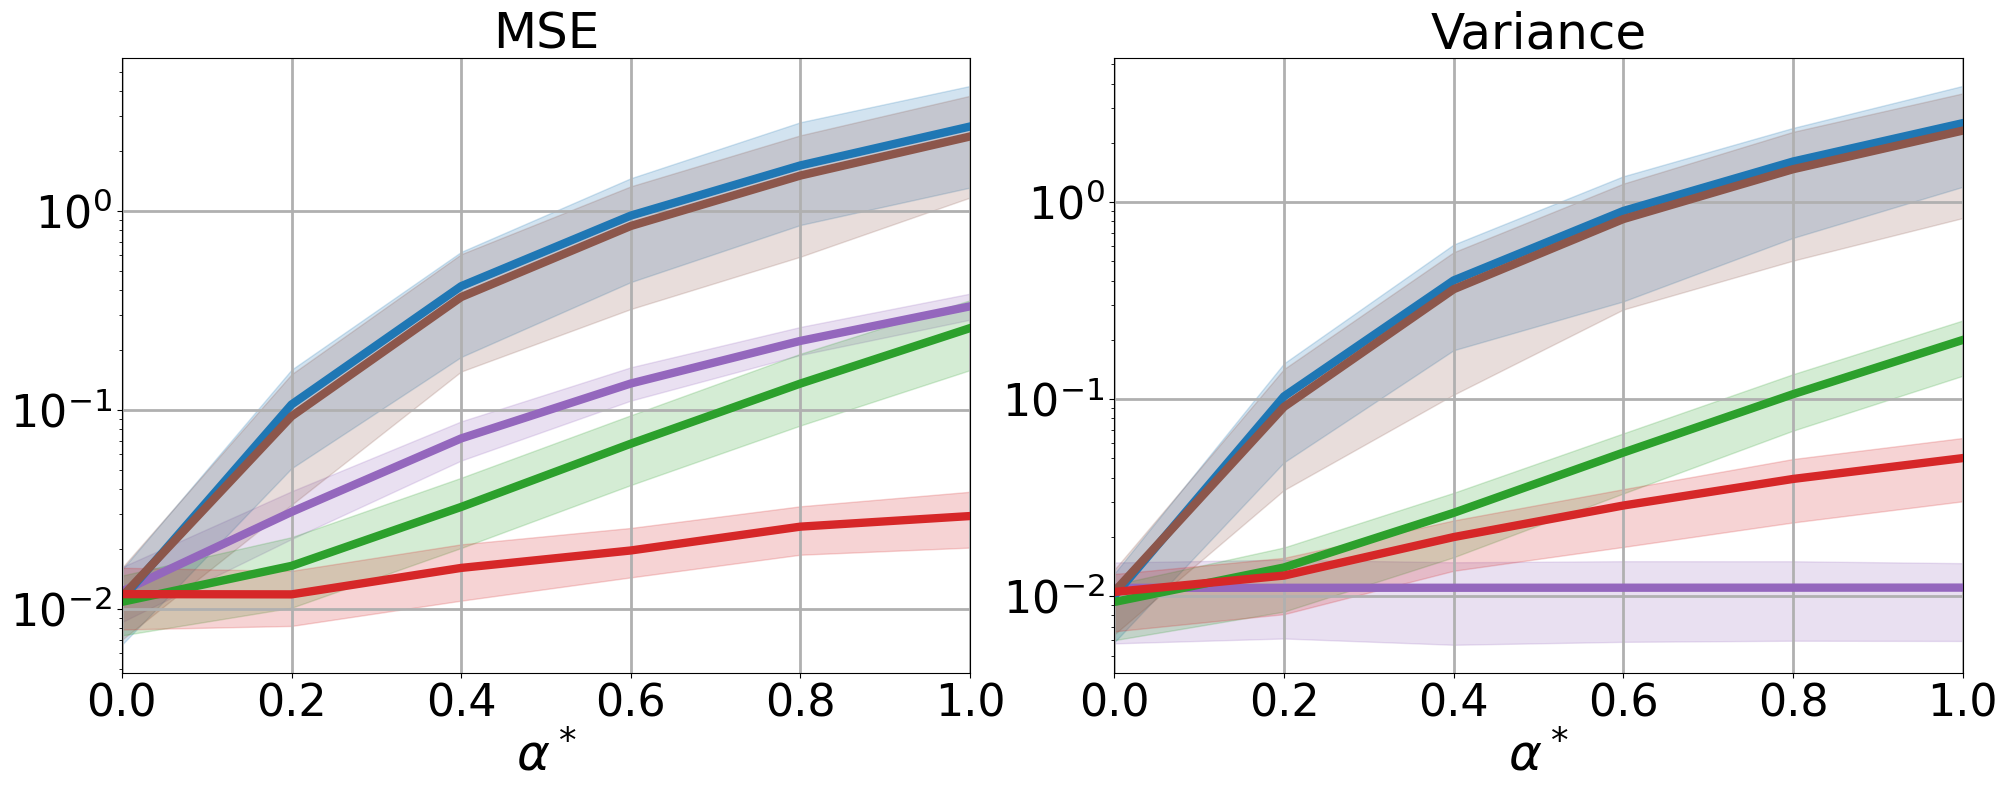
\includegraphics[height=1.06in]{figures/mr/ope_vs_alphatar_nac_100_neval_800_dimc_1000.png}
         \caption{Results with varying $\alpha^\ast$.}
         \label{fig:mse-vs-betatar}
     \end{subfigure}\\
    \caption{Results for synthetic data experiment. In \ref{fig:mse-vs-neval} we have $\alpha^\ast=0.8$ and in \ref{fig:mse-vs-betatar} we have $n = 800$.}
    \label{fig:syn_results1}
\end{figure}

% \begin{figure}[t]
%      \centering
%      \begin{subfigure}[b]{1\textwidth}
%          \centering
%          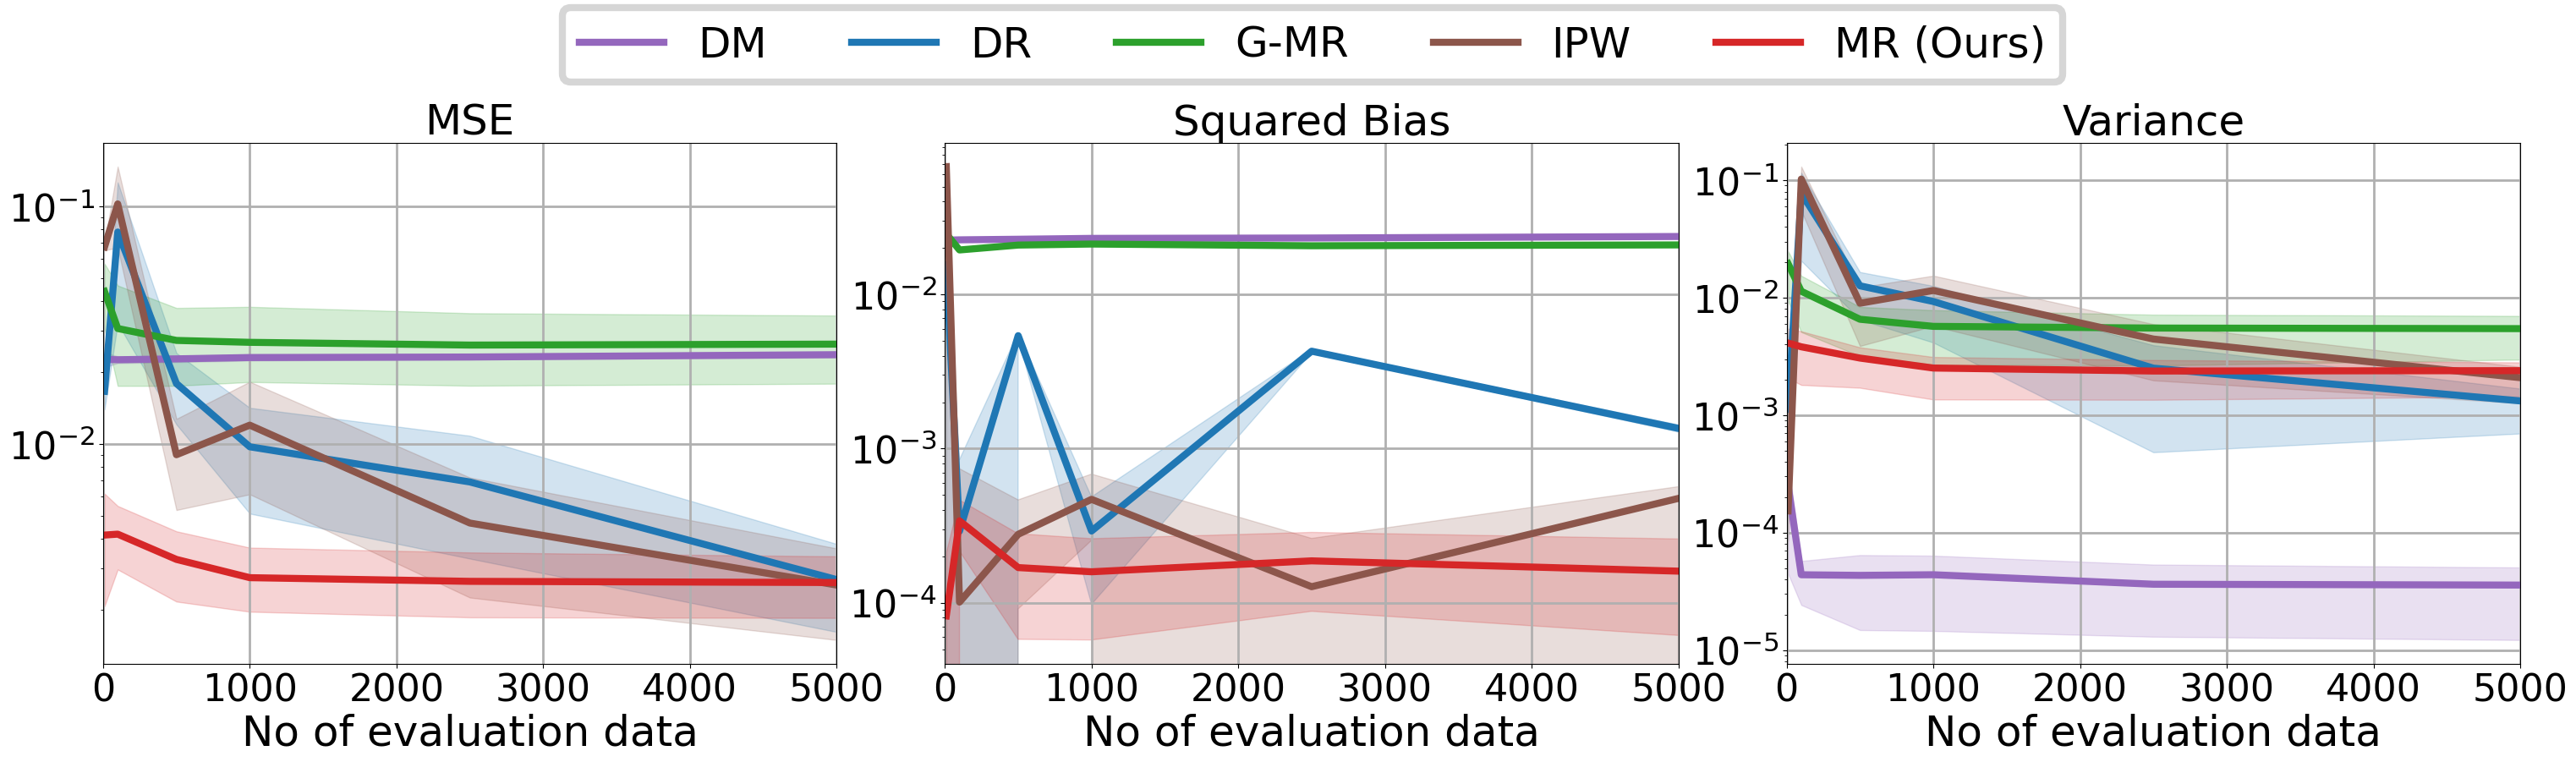
\includegraphics[width=0.75\textwidth]{figures/mr/ope_vs_neval_nac_100_alphatar_0_8_dimc_100_ntrain_100000.png}
%          \caption{Results with varying size of evaluation dataset $n$ for $\alpha^\ast = 0.8$.}
%          \label{fig:mse-vs-neval}
%      \end{subfigure}\\
%      \begin{subfigure}[b]{1\textwidth}
%          \centering
%          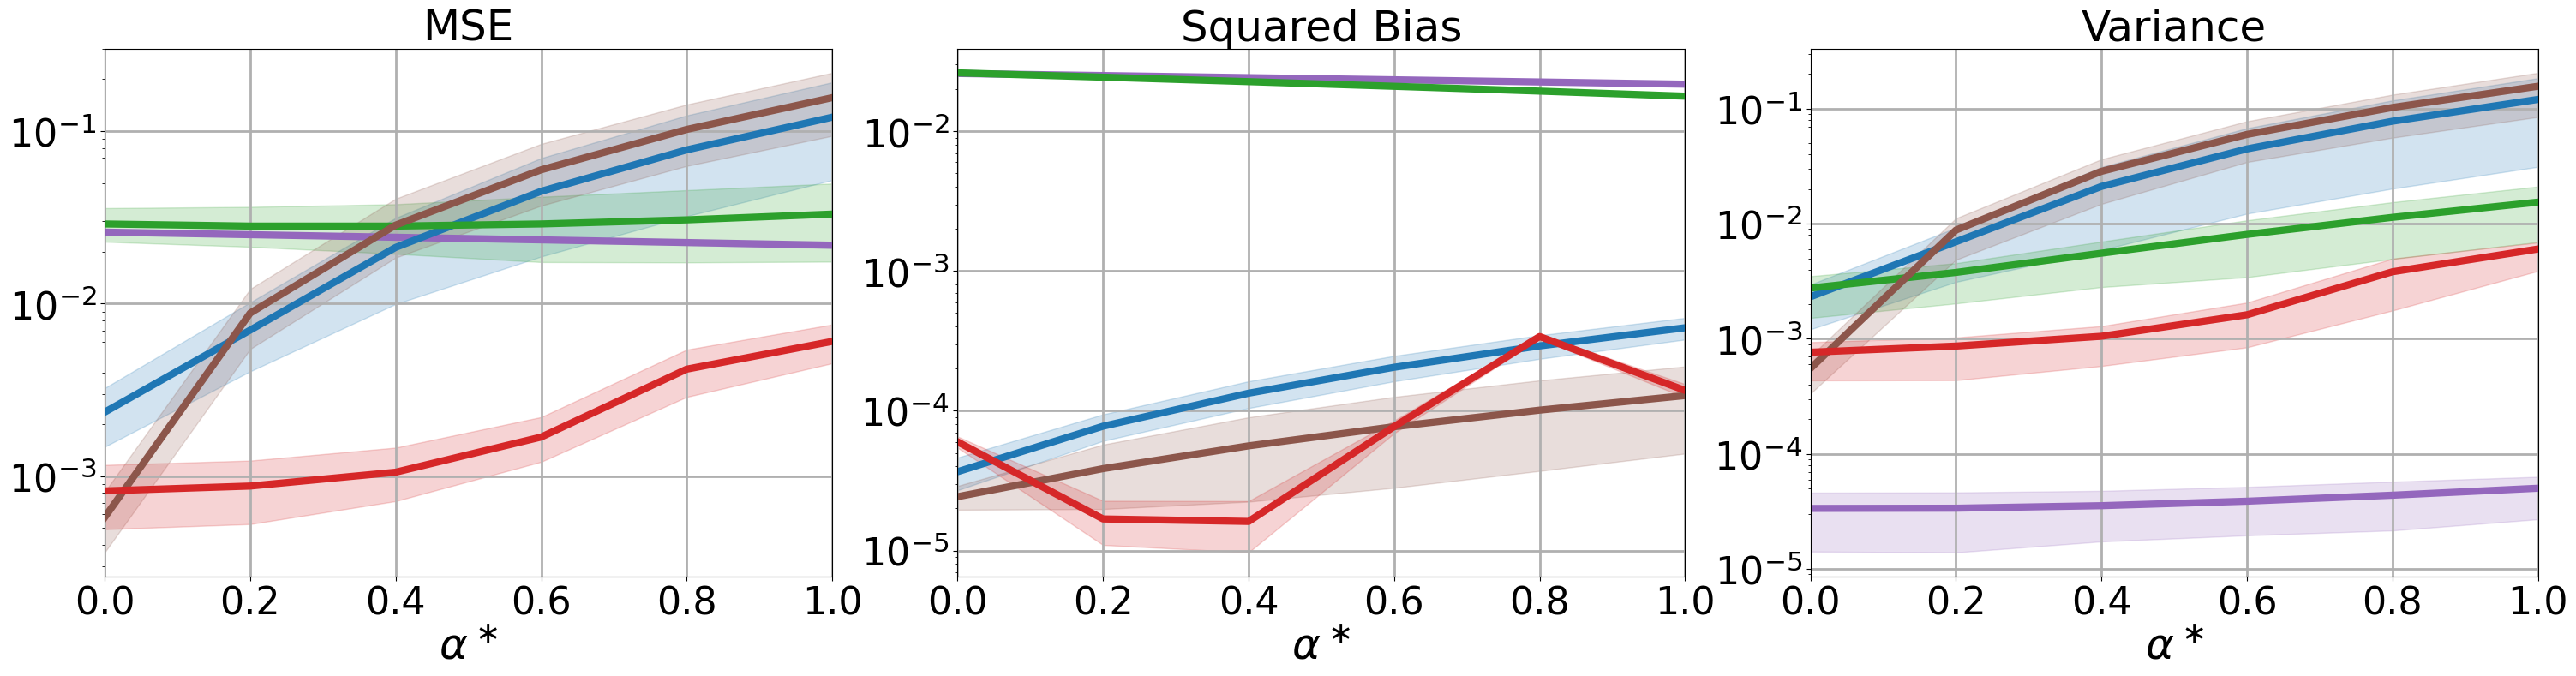
\includegraphics[width=0.75\textwidth]{figures/mr/ope_vs_alphatar_nac_100_neval_100_dimc_100_ntrain_100000.png}
%          \caption{Results with varying $\alpha^\ast$ for $n = 100$.}
%          \label{fig:mse-vs-betatar}
%      \end{subfigure}\\
%     \caption{Results with increasing $n$ and $\alpha^\ast$.}
%     \label{fig:syn_results1}
% \end{figure}
\myparagraph{Results}
We compute the target policy value using the $n$ evaluation datapoints. Here, the MSE of the estimators is computed over 10 different sets of logged data replicated with different seeds. The results presented have context dimension $d=1000$, number of actions $n_a=100$ and training data size $m=5000$. More experiments for a variety of parameter values are included in Appendix \ref{subsec:mips-empirical}.


% \begin{figure}
%      \centering
%      \begin{subfigure}[b]{1\textwidth}
%          \centering
%          \includegraphics[width=\textwidth]{figures/mr/latest/ope_vs_neval_nac_100_alphatar_0.2_dimc_100_ntrain_100000.png}
%          \caption{Results with varying size of evaluation dataset $n$ for $d=100$, $n_{a}=100$, $\alpha^\ast = 0.2$.}
%          \label{fig:mse-vs-neval}
%      \end{subfigure}\\
%      \begin{subfigure}[b]{1\textwidth}
%          \centering
%          \includegraphics[width=\textwidth]{figures/mr/latest/ope_vs_alphatar_dimc_100_nac_100_neval_100_ntrain_10000.png}
%          \caption{Results with varying $\alpha^\ast$ for $d=100$, $n_{a}=100$, $n = 100$.}
%          \label{fig:mse-vs-betatar}
%      \end{subfigure}\\
%      \begin{subfigure}[b]{1\textwidth}
%          \centering
%          \includegraphics[width=\textwidth]{figures/mr/latest/ope_vs_dimc_nac_100_alphatar_0.2_neval_100_ntrain_100000.png}
%          \caption{Results with varying context dimensions $d$ for $n_{a}=100$, $n = 100$, $\alpha^\ast = 0.2$.}
%          \label{fig:mse-vs-d}
%      \end{subfigure}\\
%      \begin{subfigure}[b]{1\textwidth}
%          \centering
%          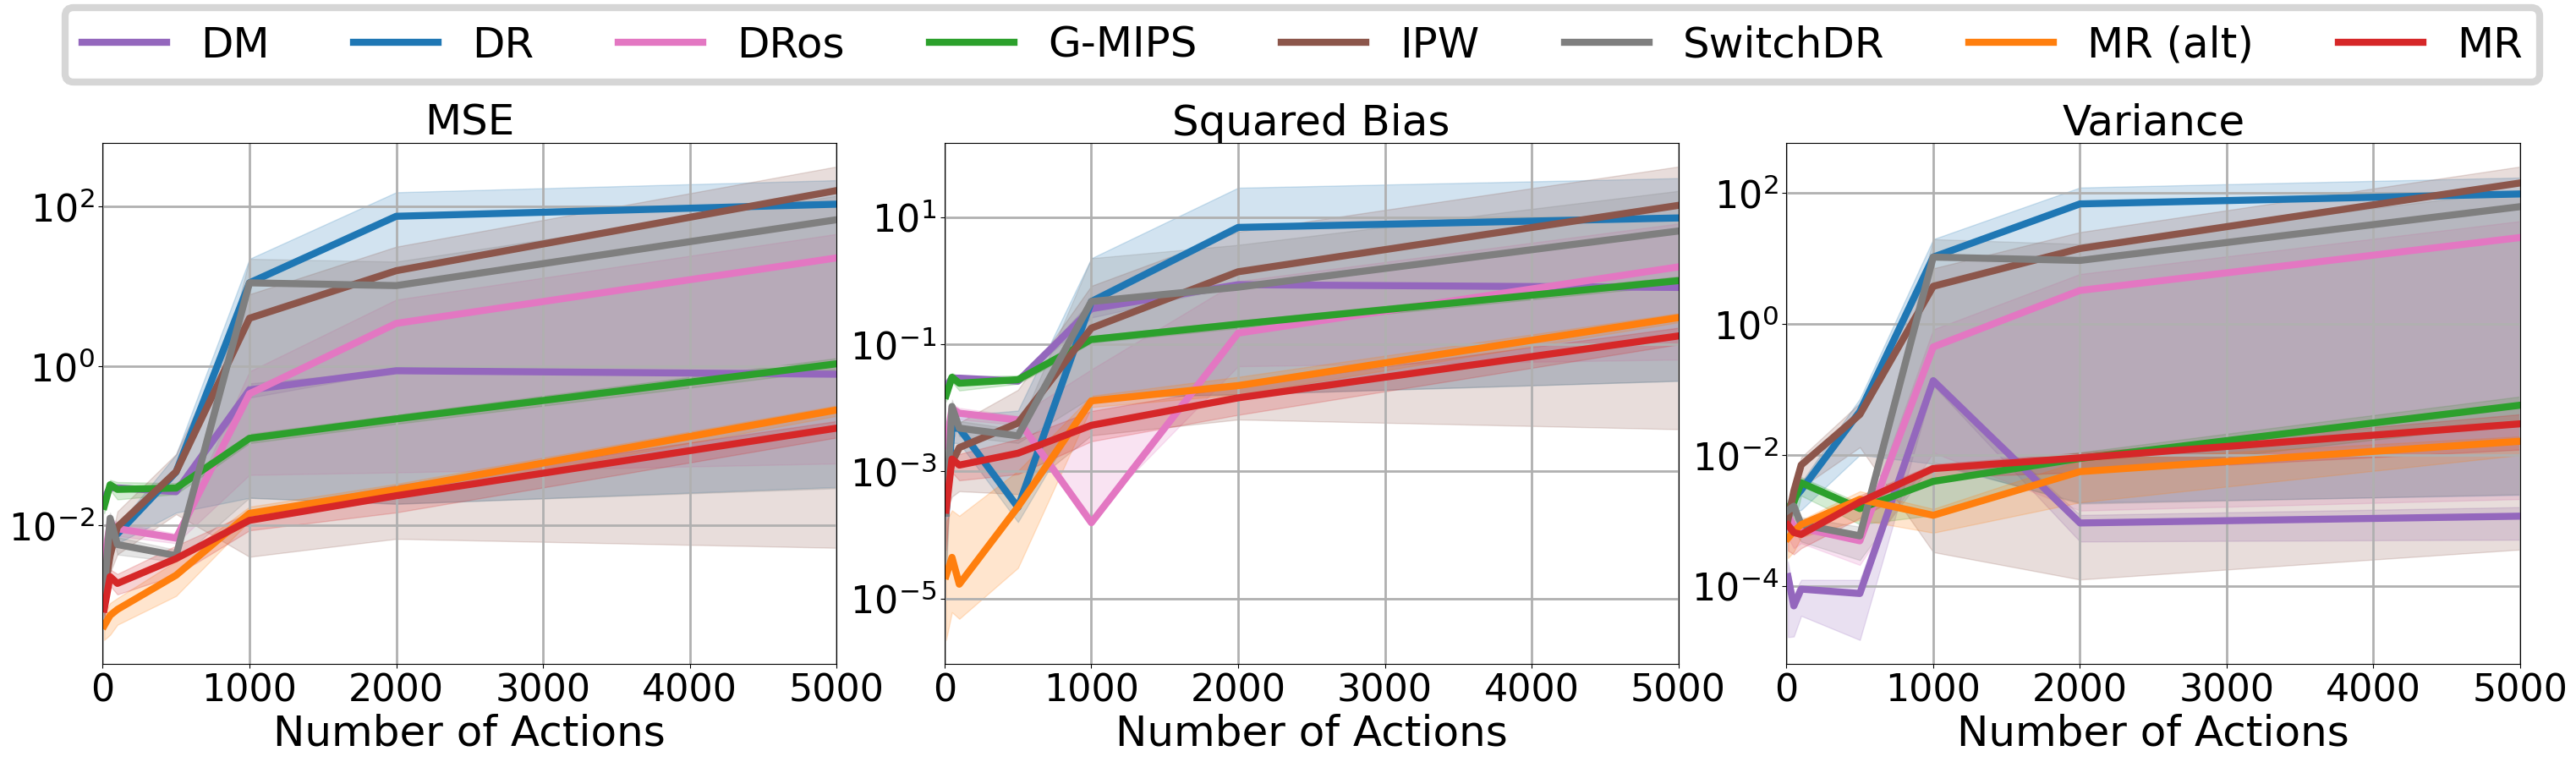
\includegraphics[width=\textwidth]{figures/mr/latest/ope_vs_nac_dimc_100_alphatar_0.2_neval_100_ntrain_100000.png}
%          \caption{Results with varying number of actions $n_{a}$ for $d=100$, $n = 100$, $\alpha^\ast = 0.2$.}
%          \label{fig:mse-vs-nac}
%      \end{subfigure}
%         \caption{Results for synthetic data experiments}
%         \label{fig:syn_results}
% \end{figure}

\myparagraph{Varying number of evaluation data $n$} 
In Figure \ref{fig:mse-vs-neval} we plot the results with increasing size of evaluation data $n$ increases. MR achieves the smallest MSE among all the baselines considered when $n$ is small, with the MSE of MR being at least an order of magnitude smaller than every baseline for $n\leq 500$. This shows that MR is significantly more accurate than the baselines when the size of the evaluation data is small. As $n\rightarrow \infty$, the difference between the results for MR and MIPS decreases. However, MR attains smaller variance and MSE than MIPS generally, verifying our analysis in Section \ref{subsec:mips-comparison}.
% IPW and DR become increasingly accurate because of their consistency and therefore the difference between MR and these baselines becomes less pronounced. 
% Additionally, it can be seen that the MR estimator also achieves the smallest squared bias overall. 
% In contrast, G-MR has a high squared bias as a result of the estimation error of the marginal ratio $\ptar(r)/\pbeh(r)$, which is more difficult to estimate the marginal ratio $\ptar(y)/\pbeh(y)$ as $r$ is two dimensional. The variance of G-MR estimator, on the other hand, is smaller than that of IPW when $n < 2000$, as suggested by Proposition \ref{prop:mips_var_reduction}.
Moreover, Figure \ref{fig:mse-vs-neval} shows that while the variance of MR is greater than that of DM, it still achieves the lowest MSE overall, owing to the high bias of DM.

\begin{wrapfigure}{r}{0.35\textwidth}
    \centering
    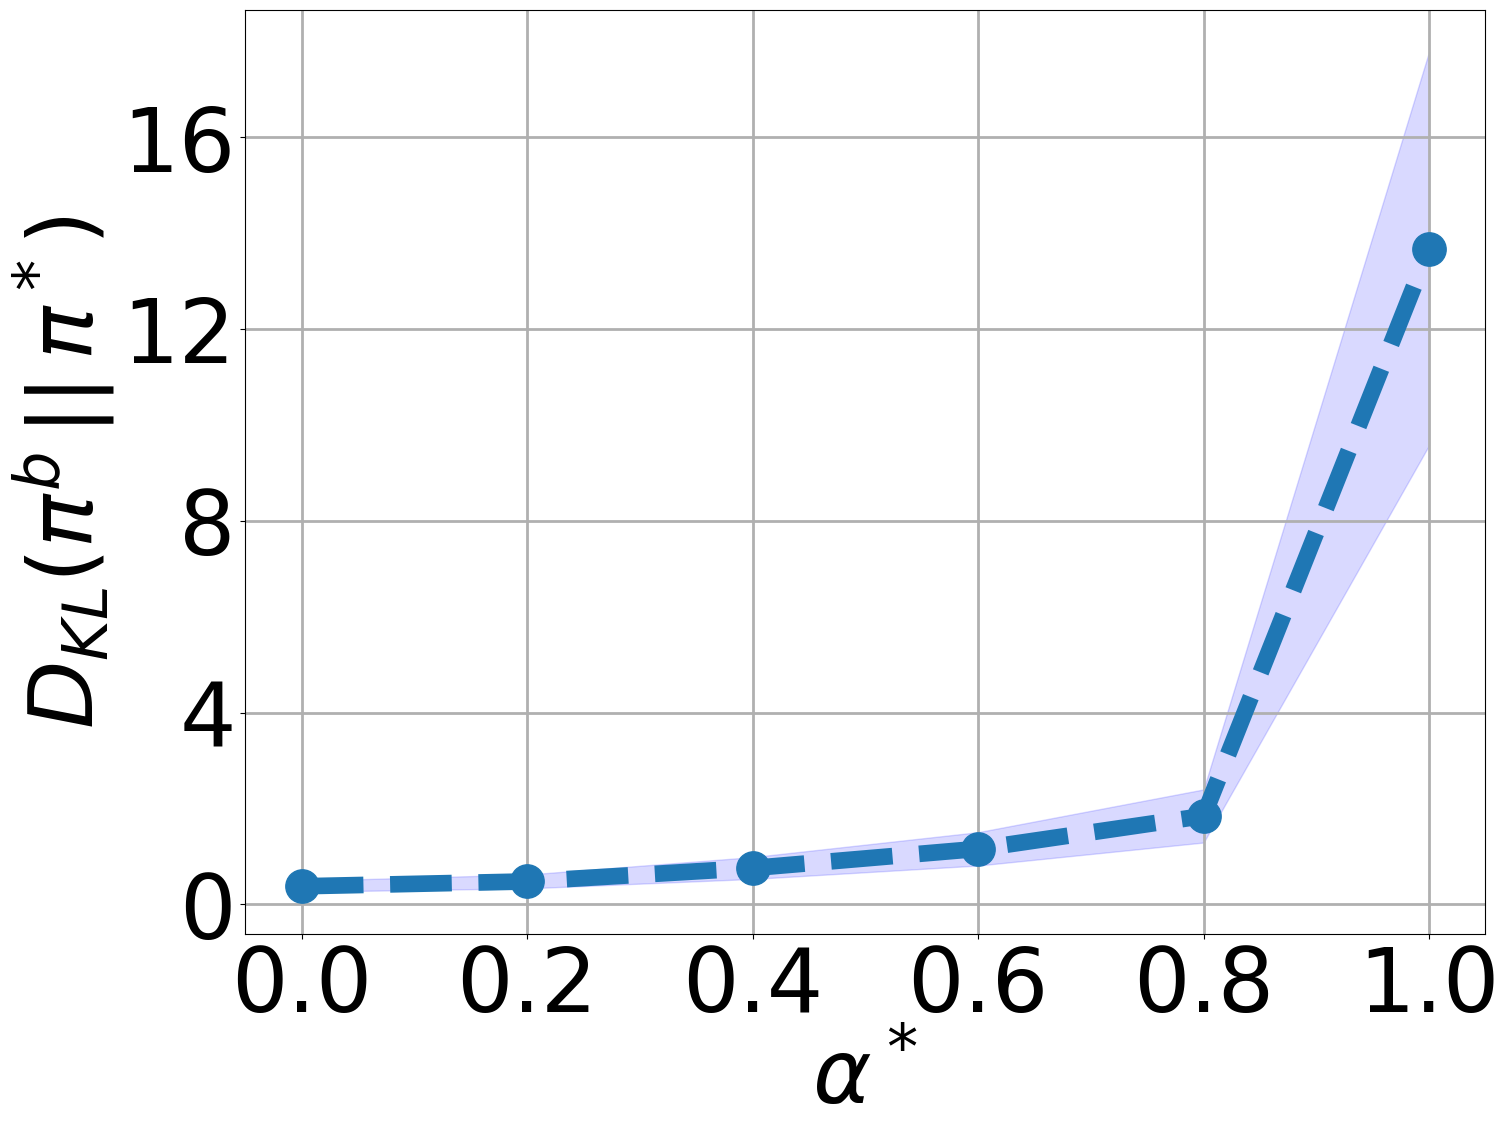
\includegraphics[width=0.35\textwidth]{figures/mr/kl-divergence-w-uncertainty.png}
    % \vspace{-0.75cm}
    % \caption{$D_{\textup{KL}}(\beh \,||\, \tar)$ with increasing $\alpha^\ast$}
    % \label{fig:kl-div-synthetic-data}
\end{wrapfigure}
\myparagraph{Varying $\alpha^\ast$}
As $\alpha^\ast$ parameter of the target policy increases, so does the shift between the policies $\beh$ and $\pi^{\alpha^\ast}$ as illustrated by the figure on the right, which plots the KL-divergence $D_{\textup{KL}}(\beh\, || \, \pi^{\alpha^\ast})$ as a function of $\alpha$.
% To analyse the shift between the policies $\beh$ and $\pi^{\alpha^\ast}$, the figure on the right plots the KL-divergence between the two policies as $\alpha^\ast$ increases. 
% \ref{fig:kl-div-synthetic-data}. 
% The figure shows that the shift between target and behaviour policies increases with increasing $\alpha^\ast$.
Figure \ref{fig:mse-vs-betatar} plots the results for increasing policy shift. 
Overall, the MSE of MR estimator is lowest among all the baselines. Moreover, while the MSE and variance of all estimators increase with increasing $\alpha^\ast$ the increase in these quantities is lower for the MR estimator than for the other baselines. Therefore, the relative performance of MR estimator improves with increasing policy shift and MR remains robust to increase in policy shift.
% It can be seen that the MSE of MR remains roughly the same with increasing $\alpha^\ast$, whereas the MSE of all other baselines increases. Moreover, both the squared bias and variance of the MR estimator becomes comparatively better than those of other baselines as the policy shift increases. 
% While the MSE and variances of all baselines increases with increasing $\beta^\ast$, the MSE and variance of MR estimator remains relatively small. Moreover, while the MSE of DM does not change noticeably with changing  $\beta^\ast$, it is still at least 2 orders of magnitude larger than that of MR. 
% This shows that MR remains significantly robust to increase in policy shift, relative to the other baselines.

\myparagraph{Additional ablation studies}
In Appendix \ref{subsec:mips-empirical}, we investigate the effect of varying context dimensions $d$, number of actions $n_a$ and number of training data $m$. In every case, we observe that the MR estimator has a smaller MSE than all other baselines considered. In particular, MR remains robust to increasing $n_a$ whereas the MSE and variance of IPW and DR estimators degrade substantially when $n_a \geq 2000$. Likewise, MR outperforms the baselines even when the training data size $m$ is small.

% \begin{figure}[t]
%      \centering
%      \begin{subfigure}[b]{0.5\textwidth}
%          \centering
%          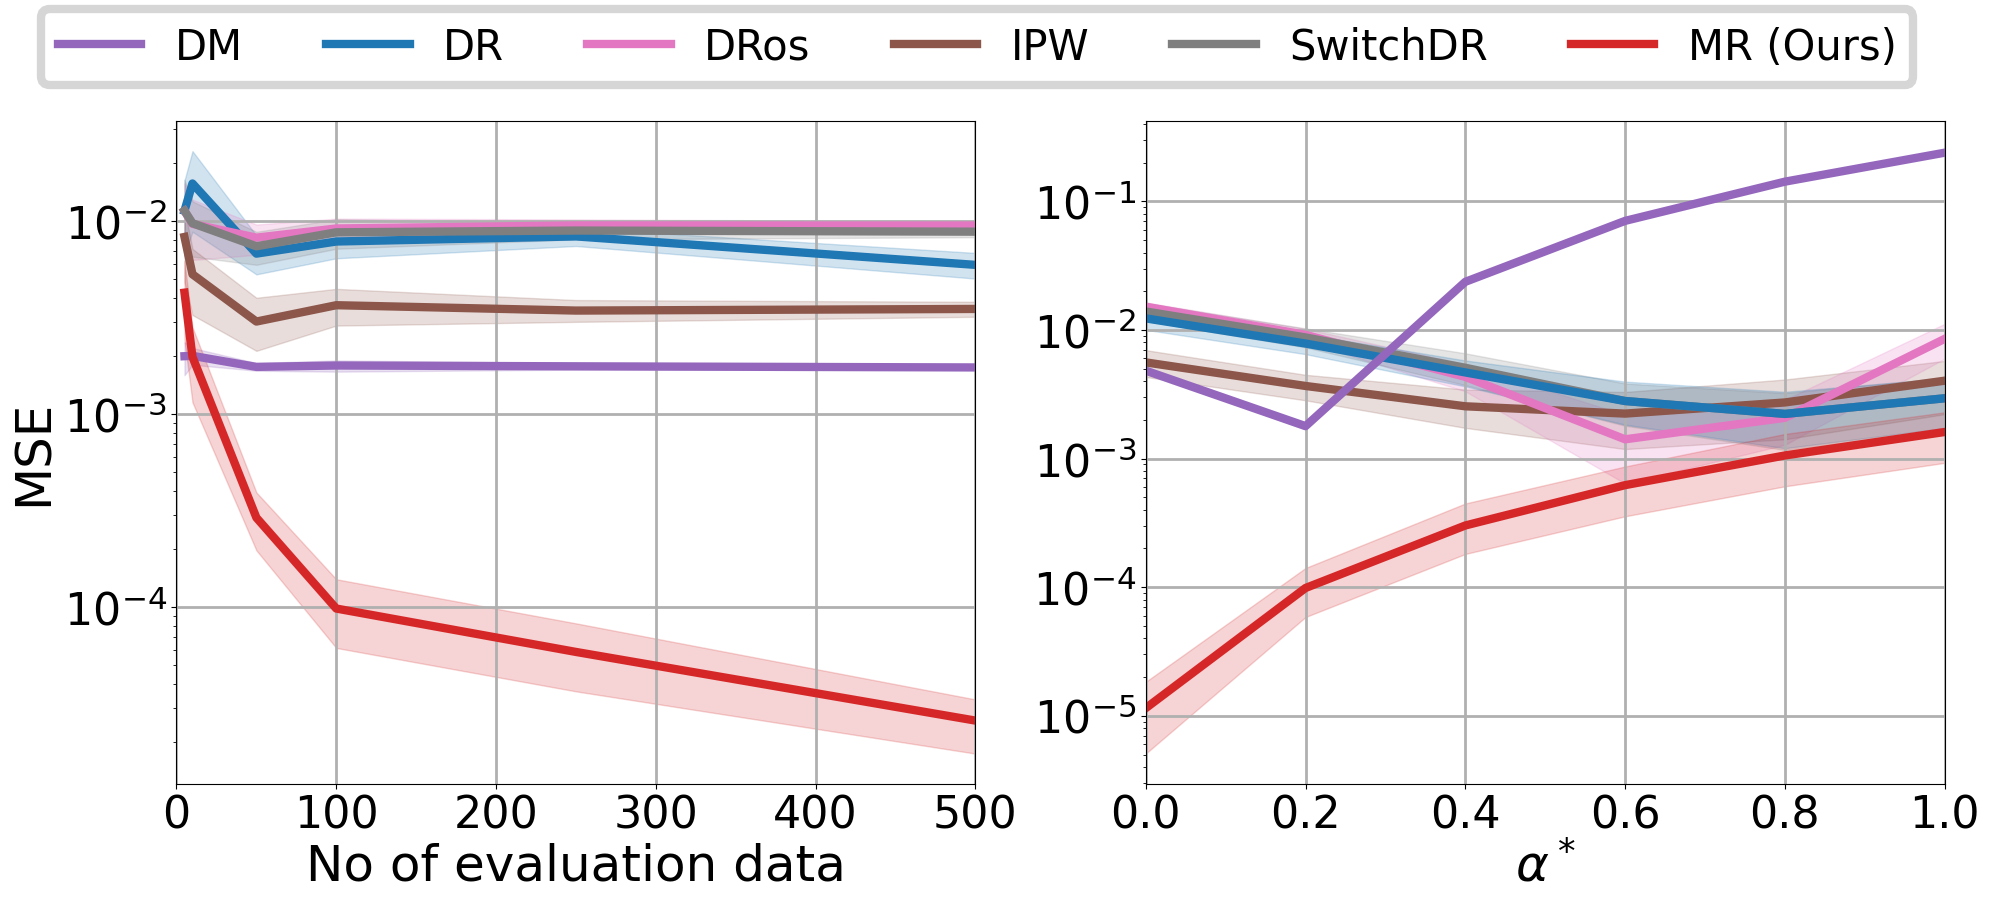
\includegraphics[height=0.92in]{figures/mr/pendigits_main.png}
%          \caption{Results for PenDigits dataset}
%          \label{fig:pendigits-main}
%      \end{subfigure}%
%      \begin{subfigure}[b]{0.5\textwidth}
%          \centering
%          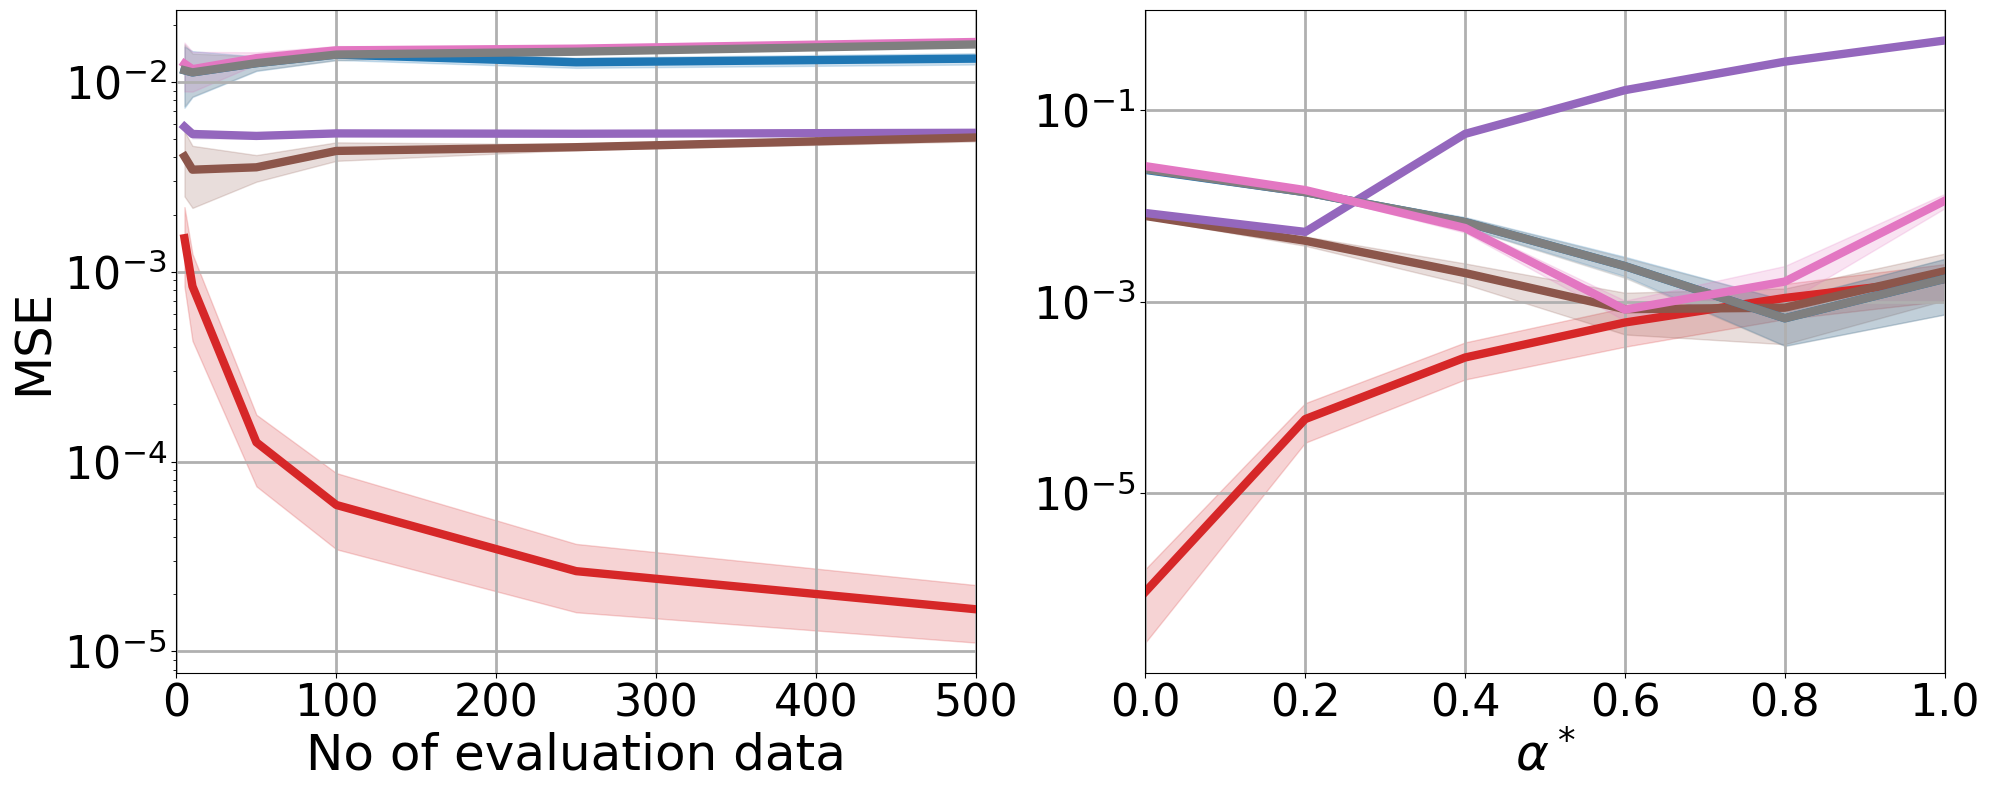
\includegraphics[height=0.92in]{figures/mr/mnist_main.png}
%          \caption{Results for mnist dataset.}
%          \label{fig:mnist-main}
%      \end{subfigure}\\
%     \caption{Results for synthetic data experiment. In \ref{fig:mse-vs-neval} we have $\alpha^\ast=0.8$ and in \ref{fig:mse-vs-betatar} we have $n = 100$.}
%     \label{fig:multiclass-main}
% \end{figure}
% \begin{table}[t]
%     \centering
%     \caption{Mean squared error of target policy value with standard errors over 10 different seeds for different classification datasets. Here, number of evaluation data $n=100$, and $\alpha^\ast=0.2$.}
%     \label{tab:classification-dataset-results}
%     \begin{tiny}
% \begin{tabular}{lllllll}
% \toprule
% Dataset & Digits & Letter & Mnist & OptDigits & PenDigits & SatImage \\
% \midrule
% DM & 0.00505$\pm$0.00016 & 0.01255$\pm$0.00011 & 0.00536$\pm$0.00009 & 0.00240$\pm$0.00009 & 0.00179$\pm$0.00011 & 0.00114$\pm$0.00005 \\
% DR & 0.01768$\pm$0.00058 & 0.00279$\pm$0.00093 & 0.01394$\pm$0.00084 & 0.00590$\pm$0.00089 & 0.00784$\pm$0.00128 & 0.02249$\pm$0.00660 \\
% DRos & 0.01721$\pm$0.00054 & 0.00281$\pm$0.00070 & 0.01467$\pm$0.00068 & 0.00788$\pm$0.00055 & 0.00916$\pm$0.00100 & 0.02160$\pm$0.00237 \\
% IPW & 0.00523$\pm$0.00030 & 0.00142$\pm$0.00062 & 0.00433$\pm$0.00044 & 0.00197$\pm$0.00035 & 0.00367$\pm$0.00077 & 0.01292$\pm$0.00455 \\
% SwitchDR & 0.01768$\pm$0.00058 & 0.00310$\pm$0.00087 & 0.01394$\pm$0.00084 & 0.00709$\pm$0.00054 & 0.00875$\pm$0.00135 & 0.02035$\pm$0.00289 \\
% MR (Ours) & \textbf{0.00011$\pm$0.00002} & \textbf{0.00020$\pm$0.00002} & \textbf{0.00006$\pm$0.00002} & \textbf{0.00025$\pm$0.00009} & \textbf{0.00010$\pm$0.00004} & \textbf{0.00014$\pm$0.00004} \\
% \bottomrule
% \end{tabular}
% \end{tiny}
% \end{table}
% \begin{table}[!htp]
%     \centering
%     \caption{Mean squared error of target policy value with standard errors over 10 different seeds for different classification datasets. Here, number of evaluation data $n=100$, and $\alpha^\ast=0.2$.}
%     \label{tab:classification-dataset-results}
%     \begin{tiny}
% \begin{tabular}{lllllll}
% \toprule
% Dataset & Digits & Letter & OptDigits & PenDigits & SatImage & Mnist \\
% \midrule
% DM & 0.00505$\pm$0.00016 & 0.01255$\pm$0.00011 & 0.00240$\pm$0.00009 & 0.00179$\pm$0.00011 & 0.00114$\pm$0.00005 & 0.00536$\pm$0.00009 \\
% DR & 0.01768$\pm$0.00058 & 0.00279$\pm$0.00093 & 0.00590$\pm$0.00089 & 0.00784$\pm$0.00128 & 0.02249$\pm$0.00660 & 0.01394$\pm$0.00084\\
% DRos & 0.01721$\pm$0.00054 & 0.00281$\pm$0.00070 & 0.00788$\pm$0.00055 & 0.00916$\pm$0.00100 & 0.02160$\pm$0.00237 & 0.01467$\pm$0.00068\\
% IPW & 0.00523$\pm$0.00030 & 0.00142$\pm$0.00062 & 0.00197$\pm$0.00035 & 0.00367$\pm$0.00077 & 0.01292$\pm$0.00455 & 0.00433$\pm$0.00044\\
% SwitchDR & 0.01768$\pm$0.00058 & 0.00310$\pm$0.00087 & 0.00709$\pm$0.00054 & 0.00875$\pm$0.00135 & 0.02035$\pm$0.00289 & 0.01394$\pm$0.00084\\
% MR (Ours) & \textbf{0.00011$\pm$0.00002} & \textbf{0.00020$\pm$0.00002} & \textbf{0.00025$\pm$0.00009} & \textbf{0.00010$\pm$0.00004} & \textbf{0.00014$\pm$0.00004} & \textbf{0.00006$\pm$0.00002}\\
% \bottomrule
% \end{tabular}
% \end{tiny}
% \end{table}
% \vspace{-5mm}
\begin{sidewaystable}[!htp]
    \centering
    \caption{Mean squared error of target policy value with standard errors over 10 different seeds for different classification datasets. Here, number of evaluation data $n=1000$, and $\alpha^\ast=0.6$.}
    \label{tab:classification-dataset-results}
    \begin{footnotesize}
    \begin{scshape}
% \begin{tabular}{lllllll}
% \toprule
% Dataset & Digits & Letter & OptDigits & PenDigits & SatImage & Mnist\\
% \midrule
% DM & 0.16053$\pm$0.00263 & 0.11686$\pm$0.00108 & 0.05963$\pm$0.00129 & 0.05889$\pm$0.00180 & 0.02165$\pm$0.00125 & 0.12556$\pm$0.00112 \\
% DR & 0.05694$\pm$0.00412 & 0.67369$\pm$0.31527 & 0.03697$\pm$0.00707 & 0.20803$\pm$0.13579 & 0.06484$\pm$0.04971 & 0.16665$\pm$0.01689 \\
% DRos & 0.03180$\pm$0.00231 & 0.05629$\pm$0.02057 & 0.00928$\pm$0.00181 & 0.00698$\pm$0.00236 & 0.00824$\pm$0.00212 & 0.06950$\pm$0.00549 \\
% IPW & 0.06465$\pm$0.00459 & 0.96803$\pm$0.44189 & 0.05451$\pm$0.00875 & 0.02769$\pm$0.00720 & 0.02298$\pm$0.00903 & 0.20363$\pm$0.02123 \\
% SwitchDR & 0.05694$\pm$0.00412 & 0.11881$\pm$0.02220 & 0.04086$\pm$0.00711 & 0.02150$\pm$0.00569 & 0.01677$\pm$0.00598 & 0.16665$\pm$0.01689 \\
% MR (Ours) & \textbf{0.00169$\pm$0.00032} & \textbf{0.00126$\pm$0.00045} & \textbf{0.00115$\pm$0.00040} & \textbf{0.00261$\pm$0.00062} & \textbf{0.00314$\pm$0.00071} & \textbf{0.00654$\pm$0.00092} \\
% \bottomrule
% \end{tabular}

\begin{tabular}{llllllll}
\toprule
Dataset &             Digits &               Letter &          OptDigits &          PenDigits &           SatImage  &              Mnist & CIFAR-100\\
\midrule
DM        &  0.1508$\pm$0.0015 &    0.0886$\pm$0.0026 &  0.0485$\pm$0.0016 &   0.0520$\pm$0.0016 &  0.0208$\pm$0.0009  &  0.1109$\pm$0.0014 & 0.0020$\pm$0.0001 \\
DR        &    0.1334$\pm$0.0400 &    \red{35.085$\pm$17.768} &  0.0464$\pm$0.0061 &  0.2343$\pm$0.1404 &   0.0560$\pm$0.0395 &  0.2617$\pm$0.0139 & \red{3823.9$\pm$2023.2} \\
DRos      &  0.0847$\pm$0.0025 &    0.2363$\pm$0.0586 &  0.0384$\pm$0.0025 &  0.0138$\pm$0.0029 &  0.0078$\pm$0.0008 &  0.2151$\pm$0.0061 & 0.2628$\pm$0.1087 \\
IPW       &  0.1632$\pm$0.0462 &  \red{45.253$\pm$22.057} &   0.0844$\pm$0.0056 &  0.1342$\pm$0.0531 &    0.0900$\pm$0.0676 & 0.3359$\pm$0.0118 & \red{4116.9$\pm$2097.9}\\
SwitchDR  &  0.0982$\pm$0.0032 &    0.2387$\pm$0.0507 &  0.0557$\pm$0.0047 &   0.0342$\pm$0.0090 &  0.0136$\pm$0.0012  &   0.2750$\pm$0.0102 & 1.1644$\pm$0.8227 \\
MR (Ours) &  \textbf{0.0034$\pm$0.0001} &    \textbf{0.0018$\pm$0.0004} &  \textbf{0.0006$\pm$0.0002} &  \textbf{0.0008$\pm$0.0002} &  \textbf{0.0016$\pm$0.0003} &  \textbf{0.0121$\pm$0.0009} &  \textbf{0.0007$\pm$0.0002}\\
\bottomrule
\end{tabular}

% \begin{tabular}{lllllll}
% \toprule
% Dataset & Digits & Letter & OptDigits & PenDigits & SatImage & Mnist\\
% \midrule
% DM & 0.161$\pm$0.003 & 0.117$\pm$0.001 & 0.060$\pm$0.001 & 0.059$\pm$0.002 & 0.022$\pm$0.001 & 0.126$\pm$0.001 \\
% DR & 0.057$\pm$0.004 & 0.674$\pm$0.315 & 0.037$\pm$0.007 & 0.208$\pm$0.136 & 0.065$\pm$0.050 & 0.167$\pm$0.017 \\
% DRos & 0.032$\pm$0.002 & 0.056$\pm$0.021 & 0.009$\pm$0.002 & 0.007$\pm$0.002 & 0.008$\pm$0.002 & 0.070$\pm$0.005 \\
% IPW & 0.065$\pm$0.005 & 0.968$\pm$0.442 & 0.055$\pm$0.009 & 0.028$\pm$0.007 & 0.023$\pm$0.009 & 0.204$\pm$0.021 \\
% SwitchDR & 0.057$\pm$0.004 & 0.118$\pm$0.022 & 0.041$\pm$0.007 & 0.022$\pm$0.006 & 0.017$\pm$0.006 & 0.167$\pm$0.017 \\
% MR (Ours) & \textbf{0.002$\pm$0.001} & \textbf{0.001$\pm$0.001} & \textbf{0.001$\pm$0.001} & \textbf{0.003$\pm$0.001} & \textbf{0.003$\pm$0.001} & \textbf{0.007$\pm$0.001} \\
% \bottomrule
% \end{tabular}
\end{scshape}
\end{footnotesize}
\end{sidewaystable}
\subsection{Experiments on classification datasets}
Following previous works on OPE in contextual bandits \citep{dudik2014doubly, kallus2021optimal, mehrdad2018more,wang2017optimal}, we transform classification datasets into contextual bandit feedback data in this experiment.
We consider five UCI classification datasets \citep{dua2019uci} as well as Mnist \citep{deng2012mnist} and CIFAR-100 \citep{krizhevsky2009learning} datasets, each of which comprises $\{(x_i, a^\gt_i)\}_{i}$, where $x_i\in \Xspace$ are feature vectors and $a^\gt_i\in \Aspace$ are the ground-truth labels.
% Here, the datasets considered include five UCI classification datasets \citep{dua2019uci}, as well as the mnist dataset \citep{deng2012mnist}. 
% Following previous works \citep{dudik2014doubly, kallus2021optimal, mehrdad2018more,wang2017optimal}, the classification datasets are transformed to contextual bandit feedback data. 
In the contextual bandits setup, the feature vectors $x_i$ are considered to be the contexts, whereas the actions correspond to the possible class of labels. For the context vector $x_i$ and the action $a_i$, the reward $y_i$ is defined as $y_i \coloneqq \ind(a_i = a^\gt_i)$, i.e., the reward is 1 when the action is the same as the ground truth label and 0 otherwise. Here, the baselines considered include the DM, IPW and DR estimators as well as Switch-DR \citep{wang2017optimal} and DR with Optimistic Shrinkage (DRos) \citep{su2020doubly}. We do not consider a MIPS baseline here as there is no natural embedding $E$ of $A$. Additional details are provided in Appendix \ref{subsec:additional-experiments-classification}. 
% regarding the behaviour and target policies and the estimation of weights are provided in Appendix \ref{sec:app-additional-results}. 
% Similar to the synthetic data experiments, we define a class of parametric target policies parameterised by $\alpha^\ast \in [0, 1]$ (i.e., $\tar = \pi^{\alpha^\ast}$). 
% However, we show in Appendix \ref{subsec:additional-experiments} that in this case, the shift between target and behaviour policies increases as $\alpha^\ast \rightarrow 0$.

In Table \ref{tab:classification-dataset-results}, we present the results with number of evaluation data $n=1000$ and number of training data $m=500$. 
The table shows that across all datasets, MR achieves the lowest MSE among all methods. \flag{Moreover, for the Letter and CIFAR-100 datasets the IPW and DR yield large bias and variance arising from poor policy estimates $\hatbeh$. Despite this, the MR estimator which utilizes the \emph{same} $\hatbeh$ for the estimation of $\hat{w}(y)$ leads to much more accurate results.} We also verify that MR outperforms the baselines for increasing policy shift and evaluation data $n$ in Appendix \ref{subsec:additional-experiments-classification}.
% In fact, the MSE of MR is at least an order of magnitude lower than that of other methods.


% We provide extensive results for increasing policy shift and evaluation data size $n$ in Appendix \ref{sec:app-additional-results}.

% We split the dataset into training and testing datasets of sizes $m$ and $n$ respectively.

% \paragraph{Reward function}
% Let $X$ be a context with ground truth label $A^\gt$, we define the reward for action $A$ as:
% \[
% Y \coloneqq \ind(A = A^\gt).
% \]

\subsection{Application to ATE estimation}\label{subsec:causal-experiments}
% Further to our discussion regarding the application of MR for ATE estimation in Section \ref{subsec:application-to-causal-inference}, 
In this experiment, we investigate the empirical performance of the MR estimator for ATE estimation. 

\myparagraph{Twins dataset}
We use the Twins dataset studied in \cite{louizos2017causal}, which comprises data from twin births in the USA between 1989-1991. The treatment $a=1$ corresponds to being born the heavier twin and the outcome $Y$ corresponds to the mortality of each of the twins in their first year of life. Specifically, $Y(1)$ corresponds to the mortality of the heavier twin (and likewise for $Y(0)$). To simulate the observational study, we follow a similar strategy as in \cite{louizos2017causal} to selectively hide one of the two twins as explained in Appendix \ref{app:ate-empirical}. We obtain a total of 11,984 datapoints, of which 5000 datapoints are used to train the behaviour policy $\hatbeh$ and outcome model $\hat{q}(x, a)$.

% Here, the baselines considered include the DM, IPW and DR estimators as well as Switch-DR \citep{wang2017optimal} and DR with Optimistic Shrinkage (DRos) \citep{su2020doubly}. We do not consider a MIPS baseline here as there is no natural embedding $E$ of $A$. 
% Results for additional baselines have been given in Appendix \ref{app:ate-empirical}. 

% \begin{wraptable}{l}{0.55\textwidth}
\begin{table}[t]
% \vspace{-4mm}
    \centering
    \caption{Mean absolute ATE estimation error $\epsilon_\ate$ with standard errors over 10 different seeds, for increasing number of evaluation data $n$.}
    \label{tab:ate_errors-main}
    \begin{small}
    \begin{tabular}{lllll}
\toprule
$n$ &             50   &             200  &             1600 &             3200 \\
\midrule
DM       &  0.092$\pm$0.003 &  0.092$\pm$0.003 &  0.092$\pm$0.004 &  0.092$\pm$0.004 \\
DR       &  0.101$\pm$0.024 &  \textbf{0.065$\pm$0.009} &  0.071$\pm$0.005 &  0.069$\pm$0.004 \\
\textsc{DRos}     &    0.100$\pm$0.017 &  0.089$\pm$0.006 &   0.093$\pm$0.004 &  0.087$\pm$0.004 \\
IPW      &  0.092$\pm$0.024 &  0.088$\pm$0.014 &  0.067$\pm$0.007 &  0.067$\pm$0.007 \\
\textsc{SwitchDR} &  0.101$\pm$0.024 &  \textbf{0.065$\pm$0.009} &  0.071$\pm$0.005 &  0.069$\pm$0.004 \\
MR (Ours)      &  \textbf{0.062$\pm$0.007} &  \textbf{0.065$\pm$0.007} &  \textbf{0.061$\pm$0.005} &  \textbf{0.061$\pm$0.006} \\
\bottomrule
\end{tabular}
\end{small}
% \vspace{-4mm}
\end{table}
% \end{wraptable}
Here, we consider the same baselines as the classification data experiments in previous section.
For our evaluation, we consider the absolute error in ATE estimation, $\epsilon_\ate$, defined as:
$
\epsilon_\ate \coloneqq | \hat{\theta}^{(n)}_\ate - \theta_\ate |.
$
Here, $\hat{\theta}^{(n)}_\ate$ denotes the value of the ATE estimated using $n$ evaluation datapoints.
%\subsubsection{Results}
We compute the ATE value using the $n$ evaluation datapoints, over 10 different sets of observational data (using different seeds). Table \ref{tab:ate_errors-main} shows that MR achieves the lowest estimation error $\epsilon_\ate$ for all values of $n$ considered here. While the performance of other baselines improves with increasing $n$, MR outperforms them all. 
% Unlike other baselines, MR uses all datapoints to estimate $\E[Y(a)]$ for $a\in \{0, 1\}$ and consequently is more data efficient. 


% \begin{figure}[t]
%      \centering
%      \begin{subfigure}[b]{1\textwidth}
%          \centering
%          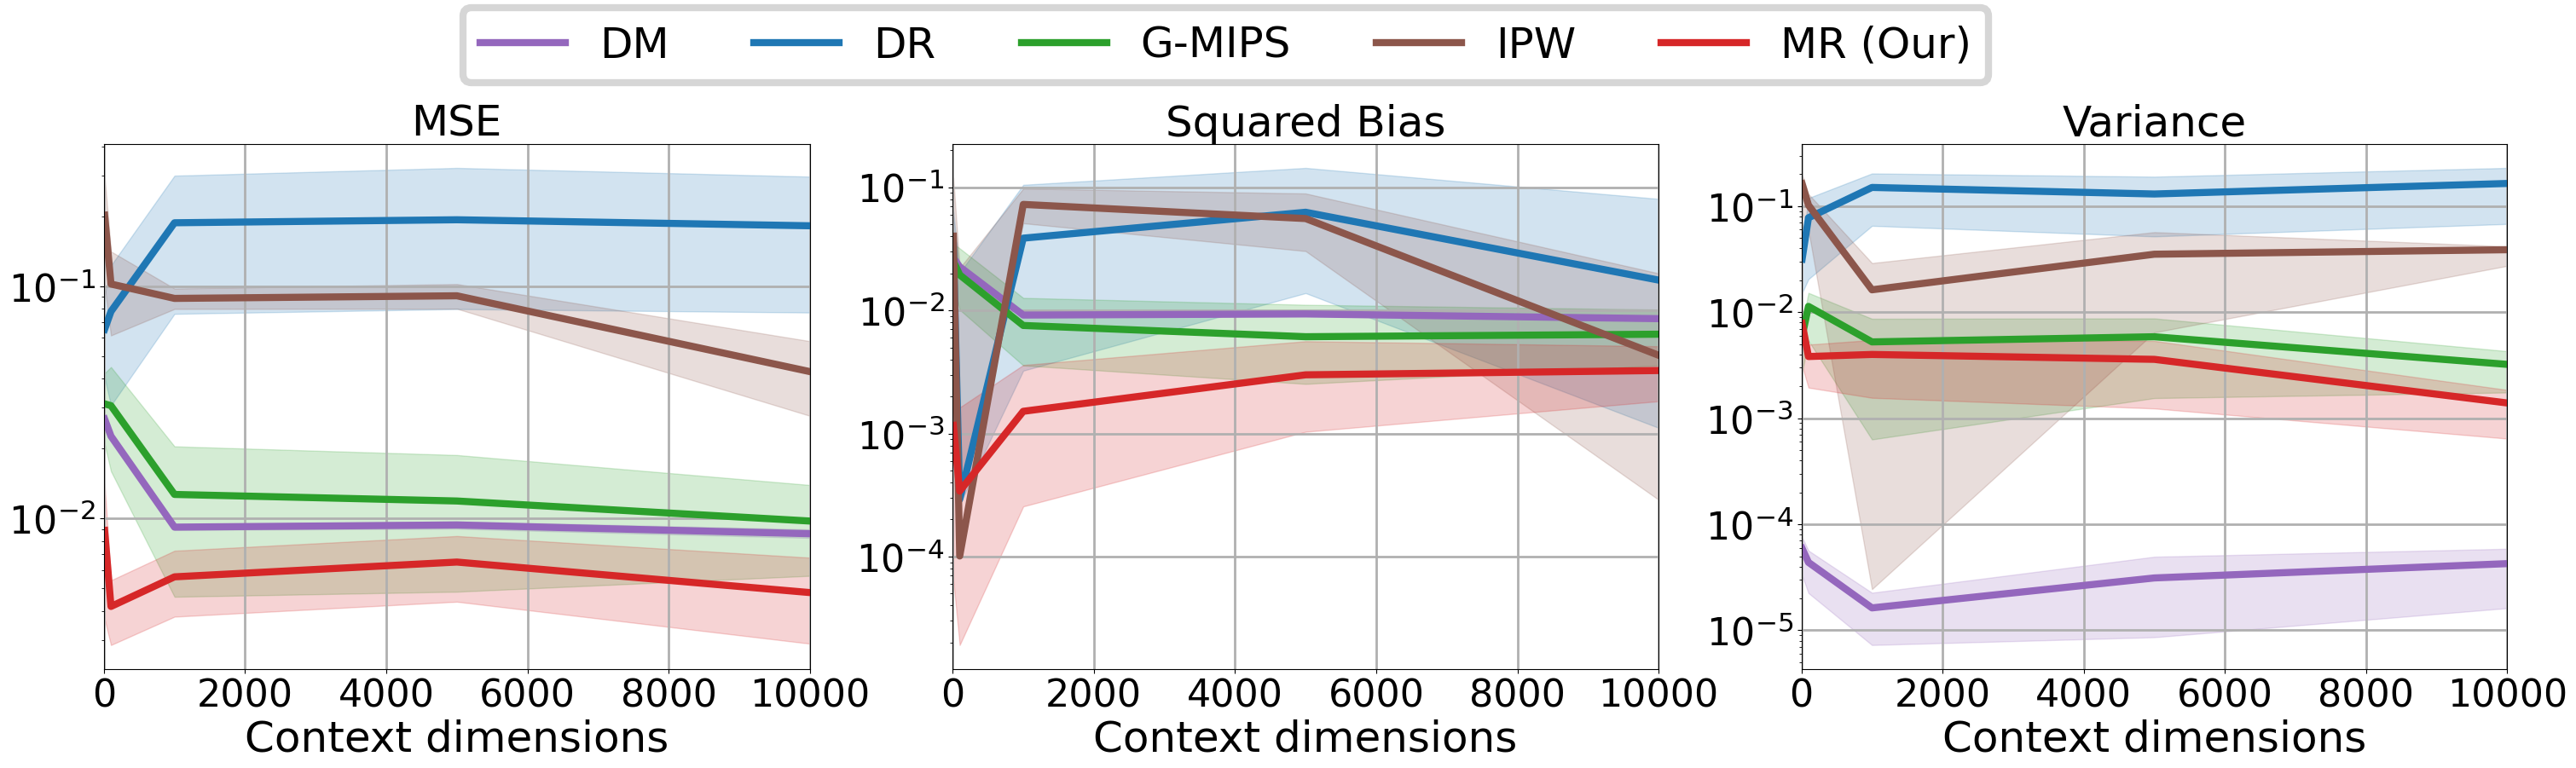
\includegraphics[width=0.75\textwidth]{figures/mr/ope_vs_dimc_nac_100_alphatar_0_8_neval_100_ntrain_100000.png}
%          \caption{Results with varying context dimensions $d$ for $n_{a}=100$, $n = 100$, $\alpha^\ast = 0.8$.}
%          \label{fig:mse-vs-d}
%      \end{subfigure}\\
%      \begin{subfigure}[b]{1\textwidth}
%          \centering
%          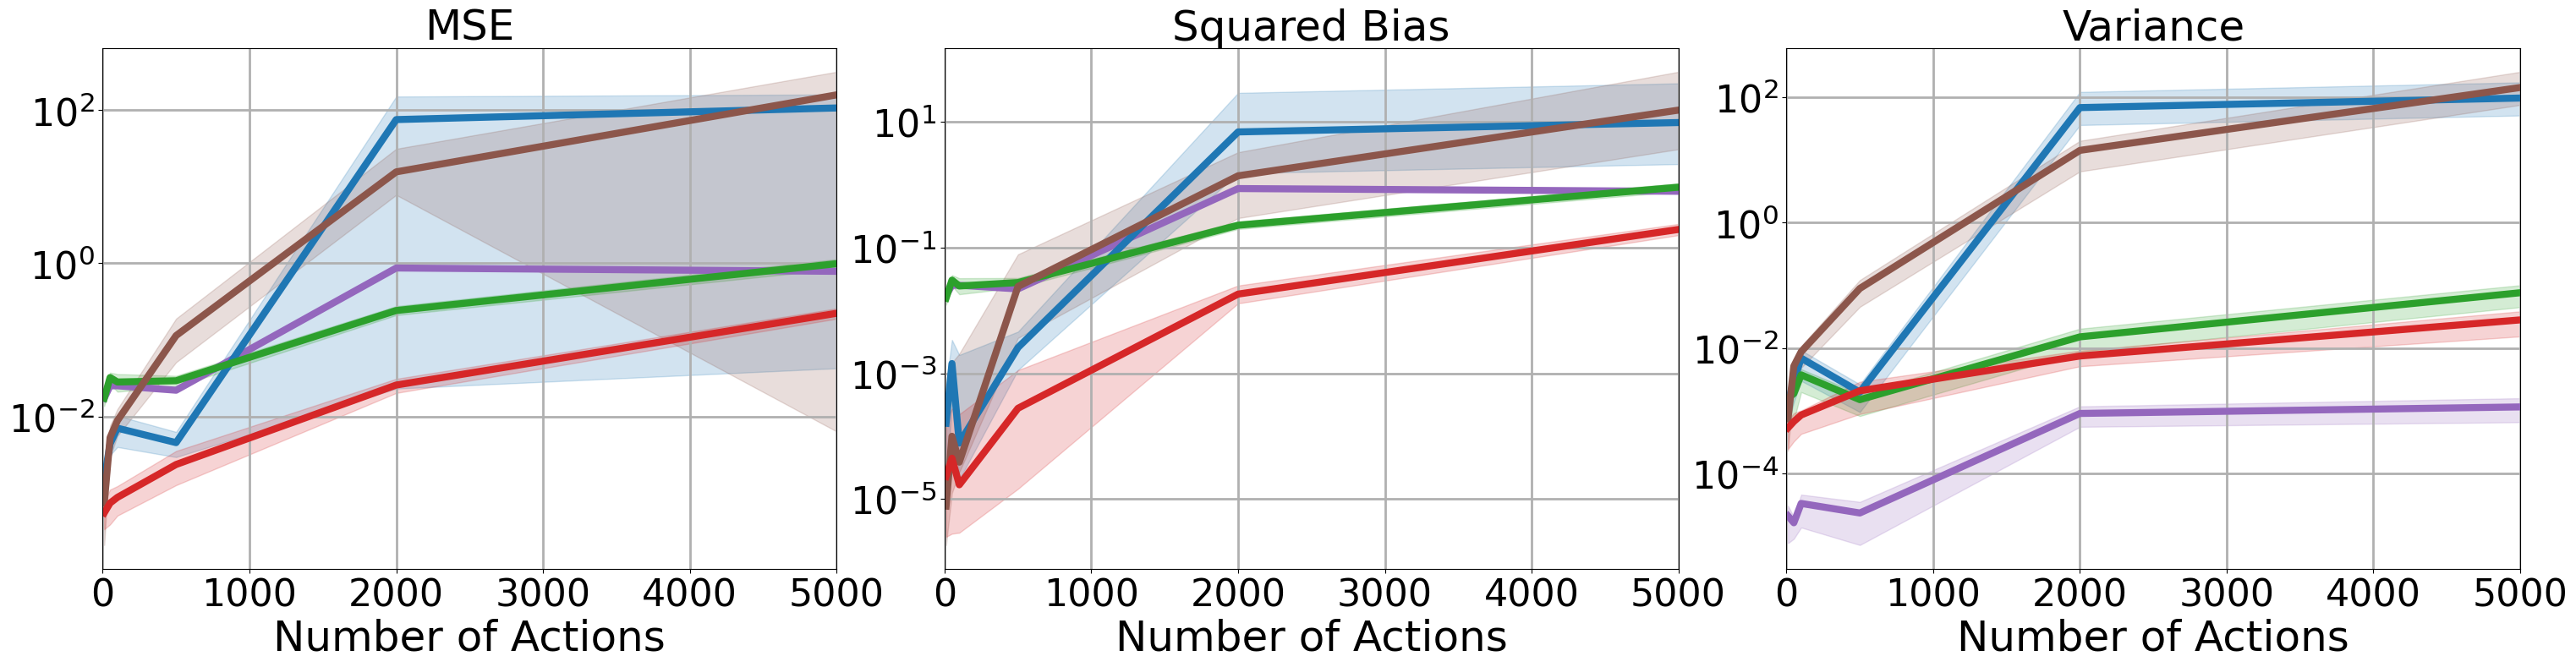
\includegraphics[width=0.75\textwidth]{figures/mr/ope_vs_nac_dimc_100_alphatar_0_2_neval_100_ntrain_100000.png}
%          \caption{Results with varying number of actions $n_{a}$ for $d=100$, $n = 100$, $\alpha^\ast = 0.2$.}
%          \label{fig:mse-vs-nac}
%      \end{subfigure}
%         \caption{Results with increasing $d$ and $n_a$.}
%         \label{fig:syn_results2}
% \end{figure}
% \paragraph{Varying $d$}
% Figure \ref{fig:mse-vs-d} plots how the results for different estimators changes as the context dimensions $d$ increases. While the results for the different baselines do not change significantly with increasing $d$, overall the MSE of MR estimator is smaller than that of other baselines.


% \paragraph{Varying $n_a$}
% Figure \ref{fig:mse-vs-nac} plots how the performance of different estimators changes as the number of actions $n_a$ increases. 
% It can be seen that the MSE and variance of IPW and DR estimators explodes when $n_a \geq 2000$. This happens because the variance of the policy ratios $\rho(a, x)$ is very large for large action spaces. In contrast, the MSE and variances of MR estimator remains relatively small even when $n_a$ is large. This shows that MR remains significantly robust in large action spaces. 

% Again, the MSE of MR estimator remains significantly smaller than the baselines with increasing values of $n_a$.
% \faaiz{think about plotting results versus the variance of policy ratios $\rho(x, a)$.}

\section{Discussion}
% \begin{itemize}
%     \item In this paper, we present marginal ratio estimator (MR) for off-policy evaluation which only considers the shift in the marginal distribution of the rewards resulting from the policy shift.
%     \item We show, theoretically and empirically, that the proposed method achieves better variance and MSE than the current SOTA methods, and is more data efficient overall.
%     \item We also show that our proposal can be used in the setting of causal inference, and provides more accurate results than the most commonly used methods.
% \end{itemize}

In this paper, we proposed an OPE method for contextual bandits called marginal ratio (MR) estimator, which considers only the shift in the marginal distribution of the outcomes resulting from the policy shift. Our theoretical and empirical analysis showed that MR achieves better variance and MSE compared to the current state-of-the-art methods and is more data efficient overall. Additionally, we demonstrated that MR applied to ATE estimation provides more accurate results than most commonly used methods. Next, we discuss limitations of our methodology and possible avenues for future work.

\myparagraph{Limitations}
The MR estimator requires the additional step of estimating $\hat{w}(y)$ which may introduce an additional source of bias in the value estimation. However, $\hat{w}(y)$ can be estimated by solving a simple 1d regression problem, and as we show empirically in Appendix \ref{app:experiments}, MR achieves the smallest bias among all baselines considered in most cases. Most notably, our ablation study in Appendix \ref{subsec:mips-empirical} shows that even when the training data is reasonably small, MR outperforms the baselines considered. 
% When the behaviour policy $\beh$ is unknown, MR estimator requires the splitting of training data to first estimate $\beh$ and subsequently to use this to estimate marginal weights $w(y)$. This data splitting can be costly in low-data settings, where we do not have access to large training datasets. However, as we empirically show in Appendix \ref{subsec:additional-experiments}, even when the training data is small, MR outperforms the baselines.  


\myparagraph{Future work}
The MR estimator can also be applied to policy optimisation problems, where the data collected using an `old' policy is used to learn a new policy. This approach has been used in Proximal Policy Optimisation (PPO) \citep{schulman2017proximal} for example, which has gained immense popularity and has been applied to reinforcement learning with human feedback (RLHF) \citep{lambert2022illustrating}. We believe that the MR estimator applied to these methodologies could lead to improvements in the stability and convergence of these optimisation schemes, given its favourable variance properties.

